\chapter{Geant4 Simulations}

In order to provide a new interactive approach to CosmicWatches for new users a scintillation simulation has been devised using the Geant4 toolkit. With this, we intend to showcase some of the physical aspects that may be studied with the detector. This project is still in development and can be found on the GitHub repository \href{https://github.com/spenceraxani/CosmicWatch_Geant4}{CosmicWatch\_Geant4}. This section aims to give a brief explanation of the inner workings of the simulation as well as the Geant4 toolkit.

\section{What is Geant4?}

As defined by the authors \cite{Geant4}, Geant4 is a simulation toolkit based in \texttt{C++}, to model the passage of particles through matter, allowing the creation of custom detector geometries, tracking, and hit recollection, including multiple physics models for processes covering a wide range of specialties, such as electromagnetic, hadronic, and optical processes. Its main areas of application are high energy, nuclear, and accelerator physics, as well as medical and space science.

A comprehensive \href{https://geant4-userdoc.web.cern.ch/UsersGuides/InstallationGuide/html/}{installation guide} has been made by the authors, the toolkit is available on Windows, MacOS, and Linux. We recommend building and installing it from source using CMake, since it provides great control over the specific configurations available during installation. Some great tutorials can also be found online, the simulations shown here are based on the architecture illustrated by Physics Matters in his YouTube series \href{https://youtube.com/playlist?list=PLLybgCU6QCGWgzNYOV0SKen9vqg4KXeVL&si=mdzOyTZS0DYsf_vc}{Geant4 Tutorials}.

\section{Geometry}

As noted before, Geant4 allows the creation of custom geometries, which in our use case is great, since it provides a platform suitable for testing multiple CosmicWatch configurations as shown in Sections \labelcref{sec:collected_produced,sec:SiPM_placement,sec:cos_squared,sec:simulated_spectra}.

In general, Geant4 requires a mother volume in which the simulation will take place, in this case, we have chosen a $10\times10\times10$ \unit{\cm\cubed} box of \texttt{G4\_AIR}\footnote{This and all other materials used in the simulation, are built from the \textit{Geant4 Material Database}, accessed through the \texttt{G4NistManager} class}. The scintillating material is a $5\times5\times1$ \unit{\cm\cubed} box of \texttt{G4\_PLASTIC\_SC\_VINYLTOLUENE}. For simplicity, the SiPM is also modeled as a box filled with \texttt{G4\_AIR} with dimensions $3\times3\times1$ \unit{\mm\cubed} attached to the base of the scintillator, this work does not yet include the electronic response of the photomultiplier. The sizes of all these elements can of course be changed (as explored in Section \labelcref{sec:collected_produced}) the settings detailed above are just the default configuration in \texttt{headers/construction.hh}. Fig. \ref{fig:geometry} shows the SiPM (\textcolor{Gray}{gray}) and scintillator (\textcolor{blue}{blue}) placement inside the mother volume (wireframe), the \textcolor{red}{red} rectangle represents the particle source.

\begin{figure}[H]
  \centering
  \begin{subfigure}[t]{0.48\textwidth}
    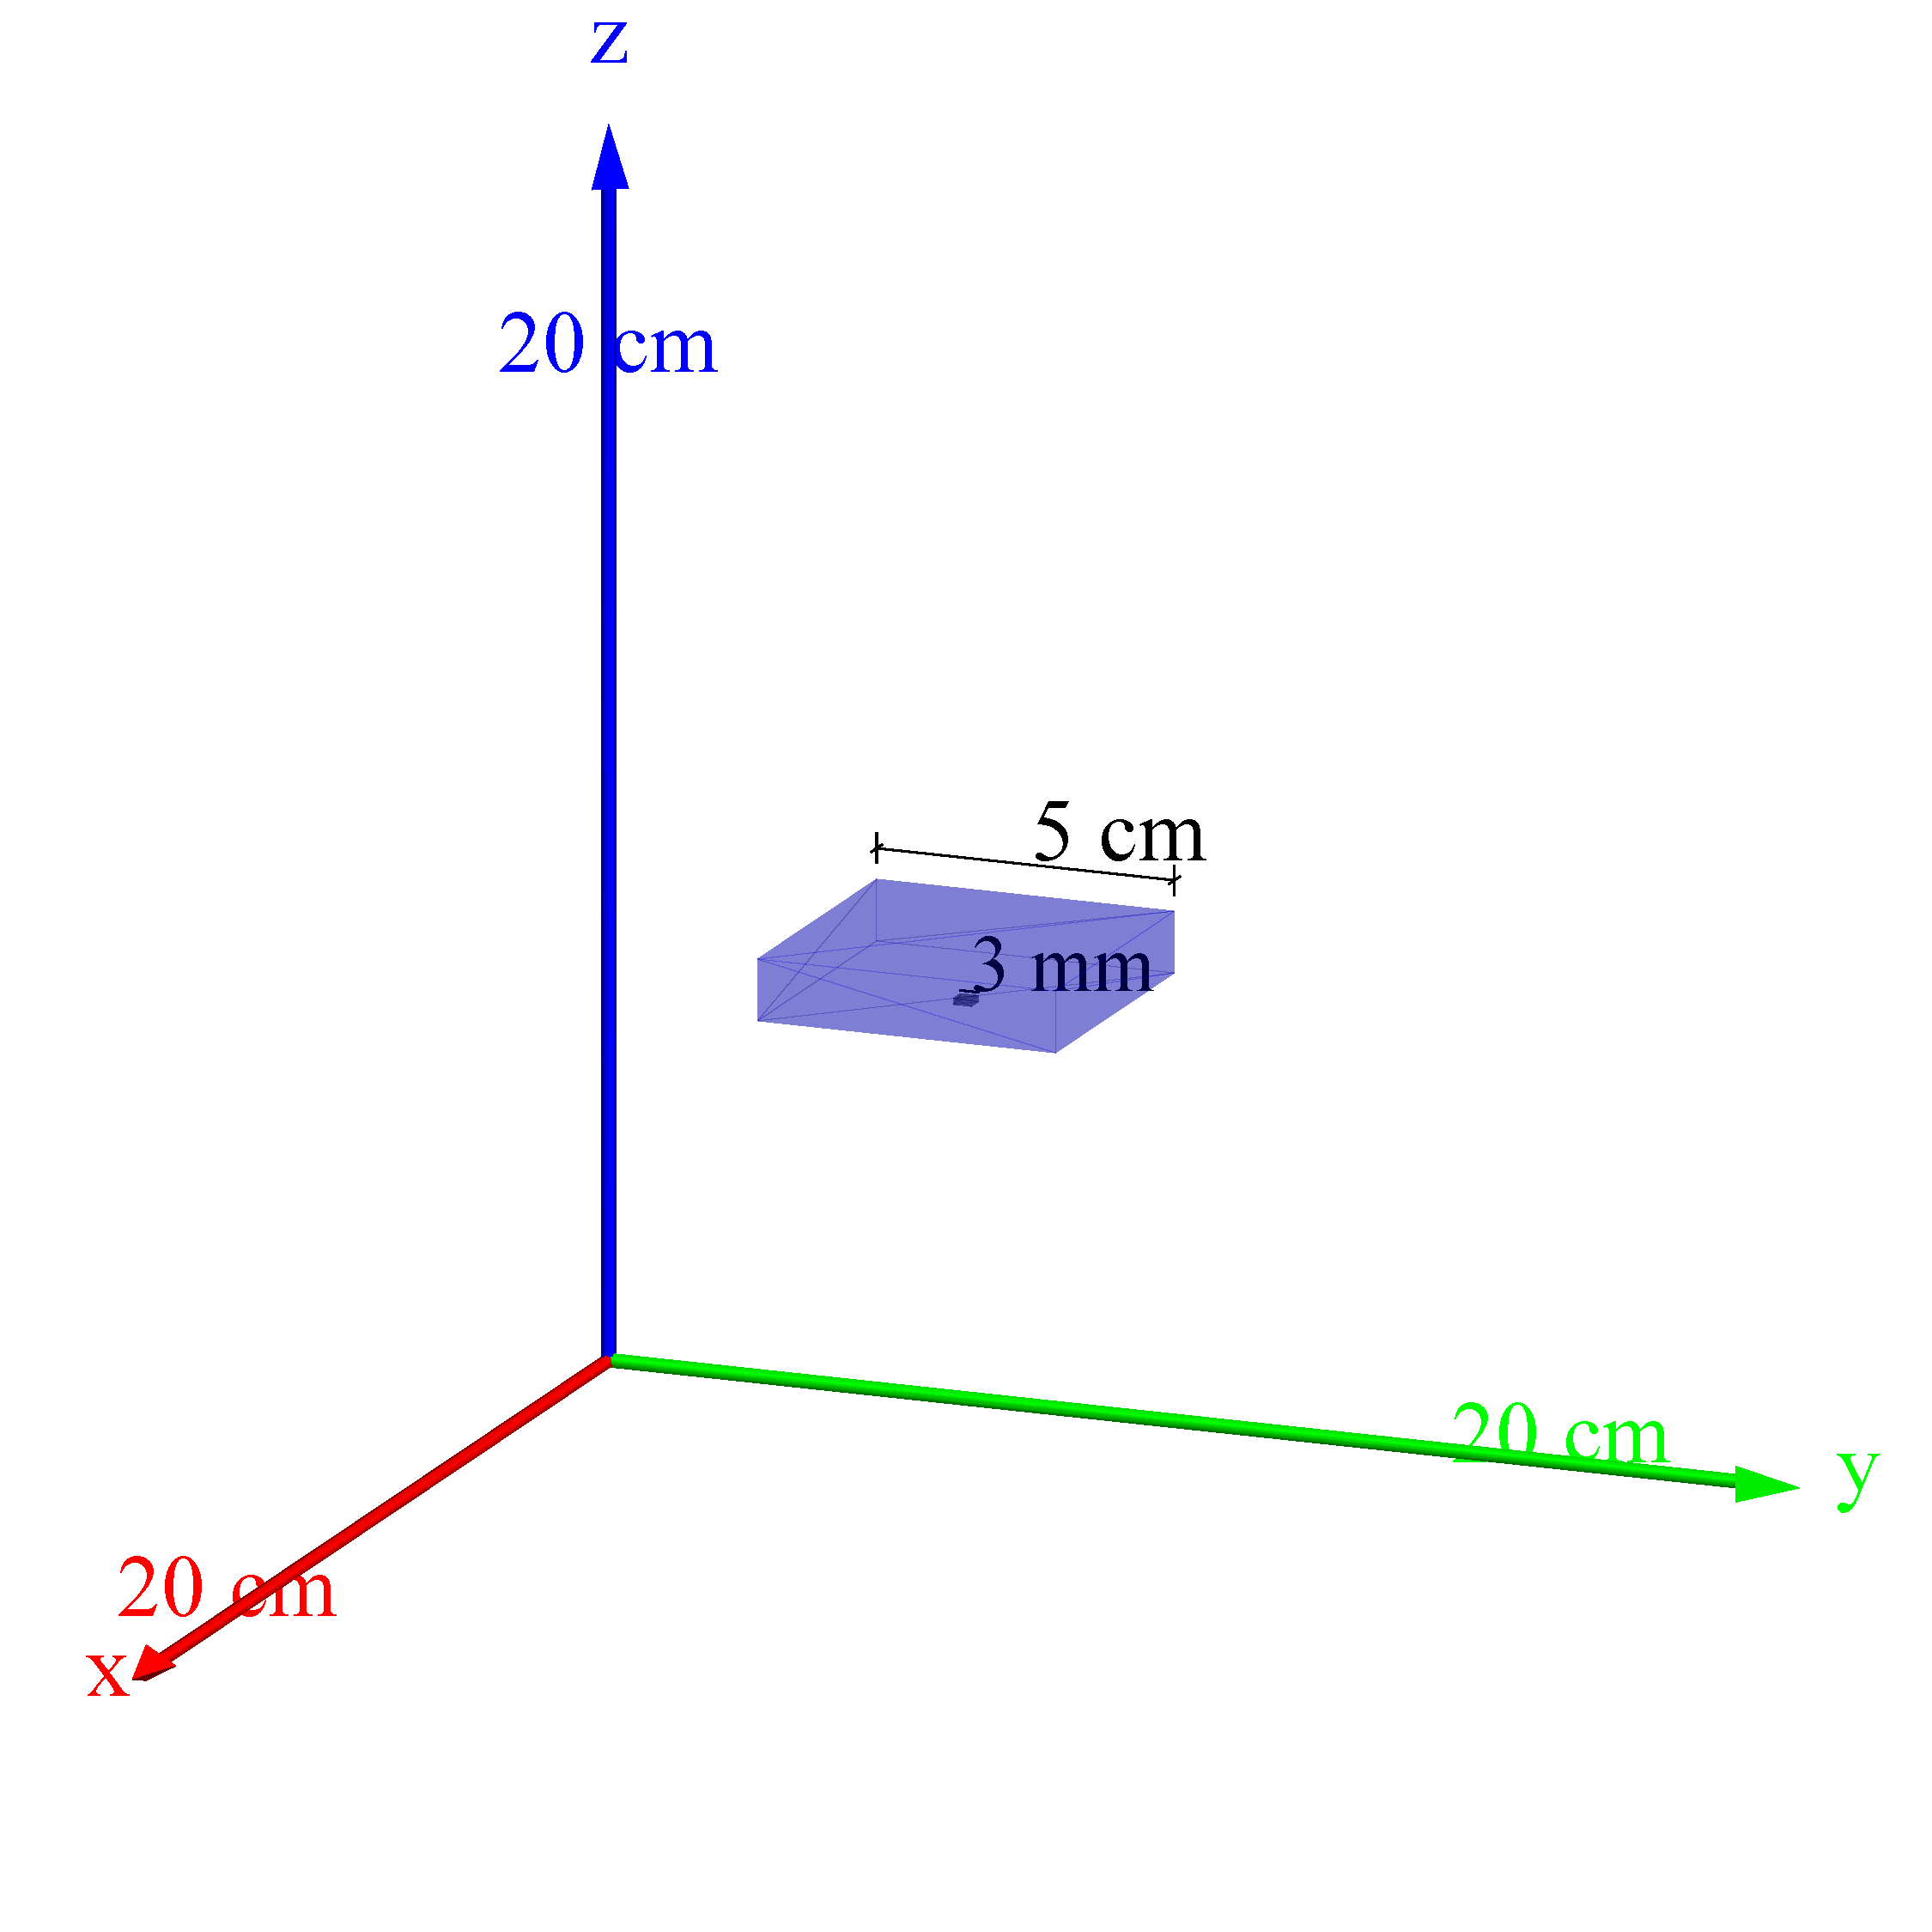
\includegraphics[width=\textwidth]{G4_simulations/profile.pdf}
    \caption{\label{sfig:geometry_profile}Diagonal view.}
  \end{subfigure}
  \hfill
  \begin{subfigure}[t]{0.48\textwidth}
    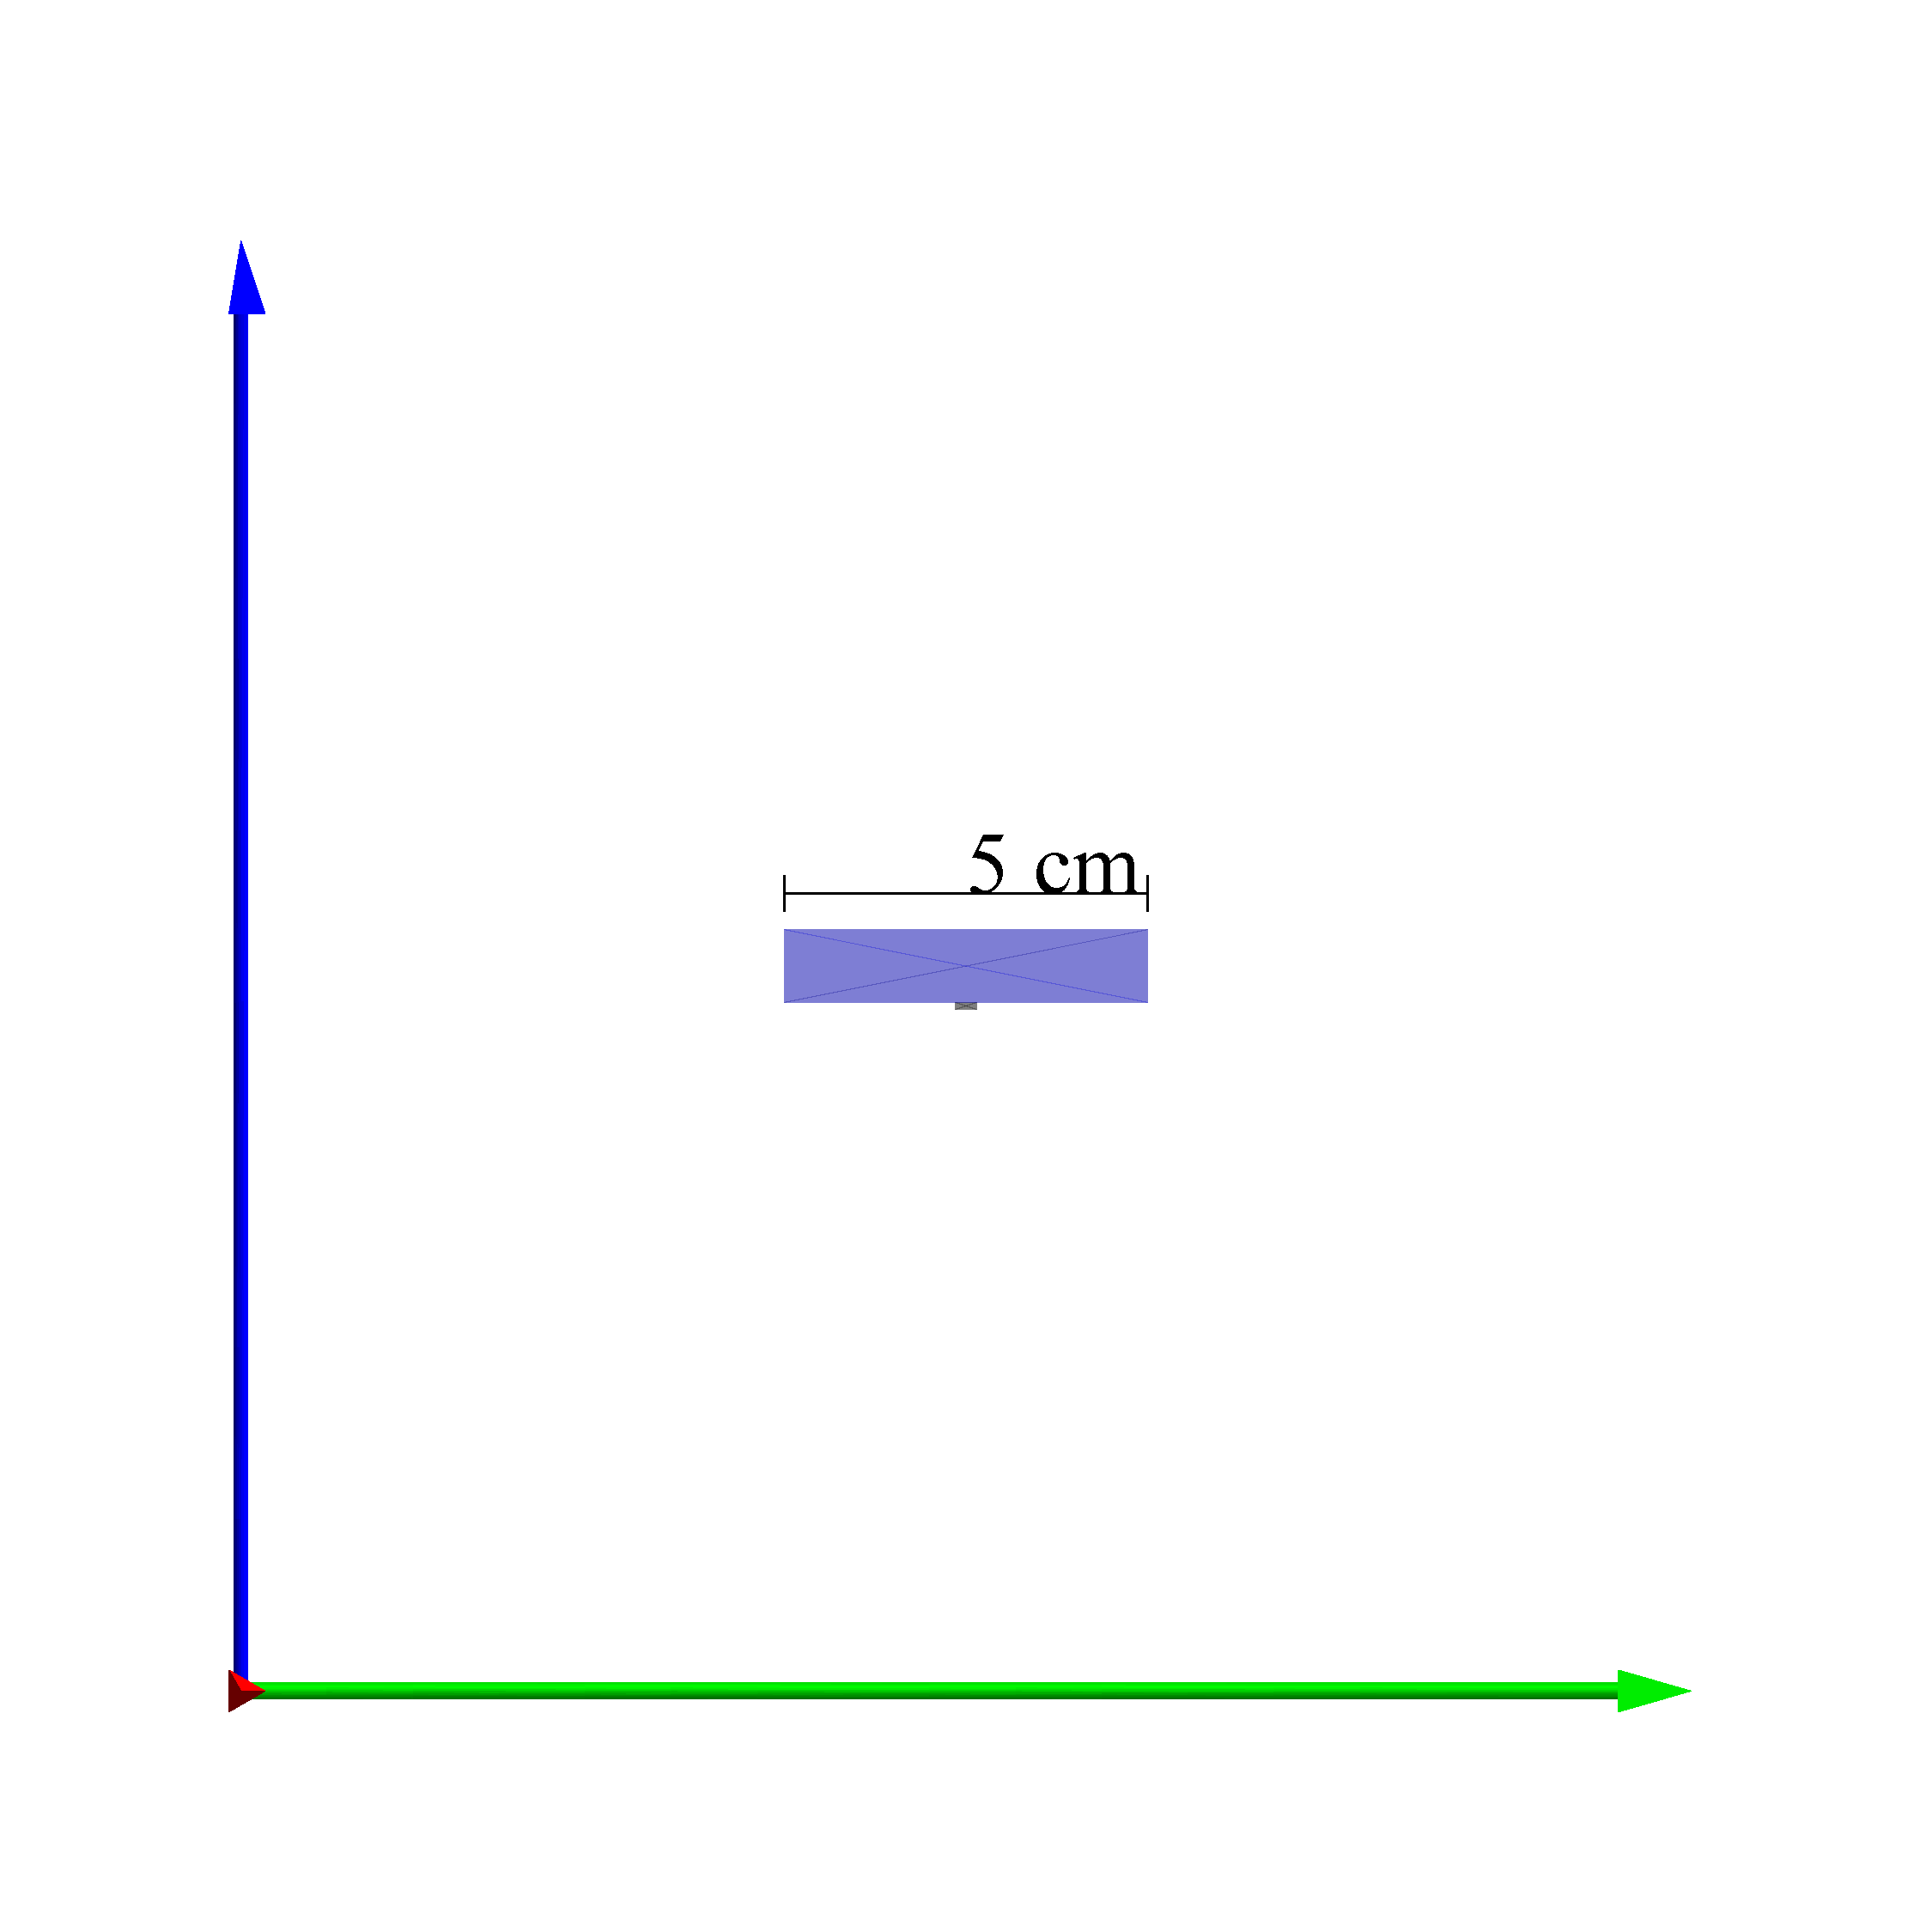
\includegraphics[width=\textwidth]{G4_simulations/front.pdf}
    \caption{\label{sfig:geometry_front}Front view.}
  \end{subfigure}
  \caption{\label{fig:geometry}Scintillator and SiPM placement in the mother volume.}
\end{figure}

\section{Simulation pipeline}

This section explains the thought process behind the simulation, illustrating the data extracted from Geant4 in order to obtain the results shown in the following Sections.

\begin{figure}[H]
  \centering
    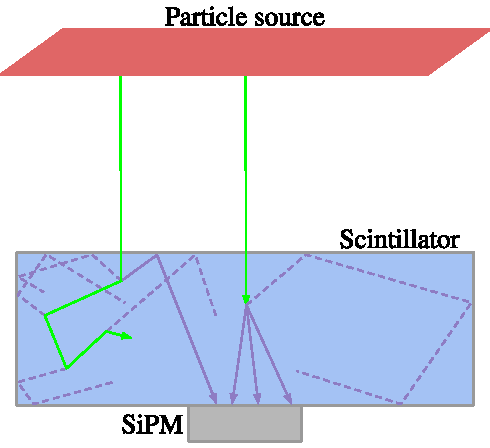
\includegraphics[width=0.47\textwidth]{G4_simulations/Simulation_pipeline.pdf}
  \caption{\label{fig:sim_pipeline}Graphic representation of the inner workings of the simulation, gamma rays are shown in \textcolor{green}{green} and optical photons in \textcolor{Orchid}{purple}.}
\end{figure}

Throughout this Chapter, an event is understood as the emission of one particle from the particle source (\gps)\footnote{The particle gun used in this simulation is a \texttt{G4GeneralParticleSource}, it can be customized through macro commands, allowing to change particle type, energy, angular distribution, and source shape among other features.} and the subsequent interactions that may occur. Figure \ref{fig:sim_pipeline} shows two different events, producing gamma rays (\textcolor{green}{green}) with the same energy, in both cases all the energy is deposited in the crystal and 5 optical photons (\textcolor{Orchid}{purple}) are produced. In the case of the gamma ray on the left, by chance, only one of the produced photons reaches the SiPM; while on the right, three of the produced photons make their way into the photomultiplier. With this in mind, for every event the simulation records:
\begin{itemize}
  \item Energy deposition in the scintillator.
  \item Number of optical photons produced.
  \item Optical photon count inside the SiPM.
  \item Angle of incidence of the original particle emitted by the \gps.
\end{itemize}

This data is then analyzed to understand the consequences of some possible choices in the detector construction, such as SiPM placement and scintillator size, along with other interesting measurements that illustrate the physical aspects of the detector.

\section{Simulation results}

The following simulations were designed to study some detector characteristics that should be taken into account while building and designing new CosmicWatches, hopefully giving insights into advantageous setups for new users. In order to speed up the simulation the \gps~ produces 50 \unit{\mega\eV} muons, this energy is much lower than what would be expected at sea level (4 \unit{\giga\eV}), but it is still useful to illustrate some interesting results.

\subsection{Photons detected vs. produced}\label{sec:collected_produced}

As showcased in Fig. \ref{fig:sim_pipeline}, not all photons reach the SiPM, The detected photons specified in the following subsections are counted as they are created (photon production) or enter the SiPM volume (photon detection). The checking process is done in \texttt{source/stepAction.cc} and relevant information for every event is saved to a \texttt{ntuple} by the Geant4 class\\ \texttt{G4GenericAnalysisManager} class as defined in \texttt{source/eventAction.cc}. The simulation speed could be improved by employing the \texttt{G4VHits} and \texttt{G4THitsCollection} classes, which are optimized to record data for every step inside a sensitive volume in the simulation.

The upper graph in Figure \ref{fig:LYSO_PScint_phot_count} shows a histogram of energy depositions in the crystal after a 50 \unit{\mega\eV} muon hits it, in this case, it is clear that the bigger crystal gets higher energy depositions, this is due to the longer travel path the muon has to go through before leaving the material. Notably, however, higher energy depositions do not necessarily correlate with higher photon counts in the SiPM. As can be seen in the bottom graph, the bigger crystal also produces more photons, since the expected light output should be proportional to the energy deposition, as explained in Section \ref{sec:simulated_spectra}, the photon production has an almost identical distribution. The photons that reach the SiPM on the other hand, are one order of magnitude below the originally produced, this is due to the attenuation length of optical photons in the material, which in this case is set to 1.6 \unit{\m} \cite{Luxium_plastic}.

\begin{figure}[H]
  \centering
  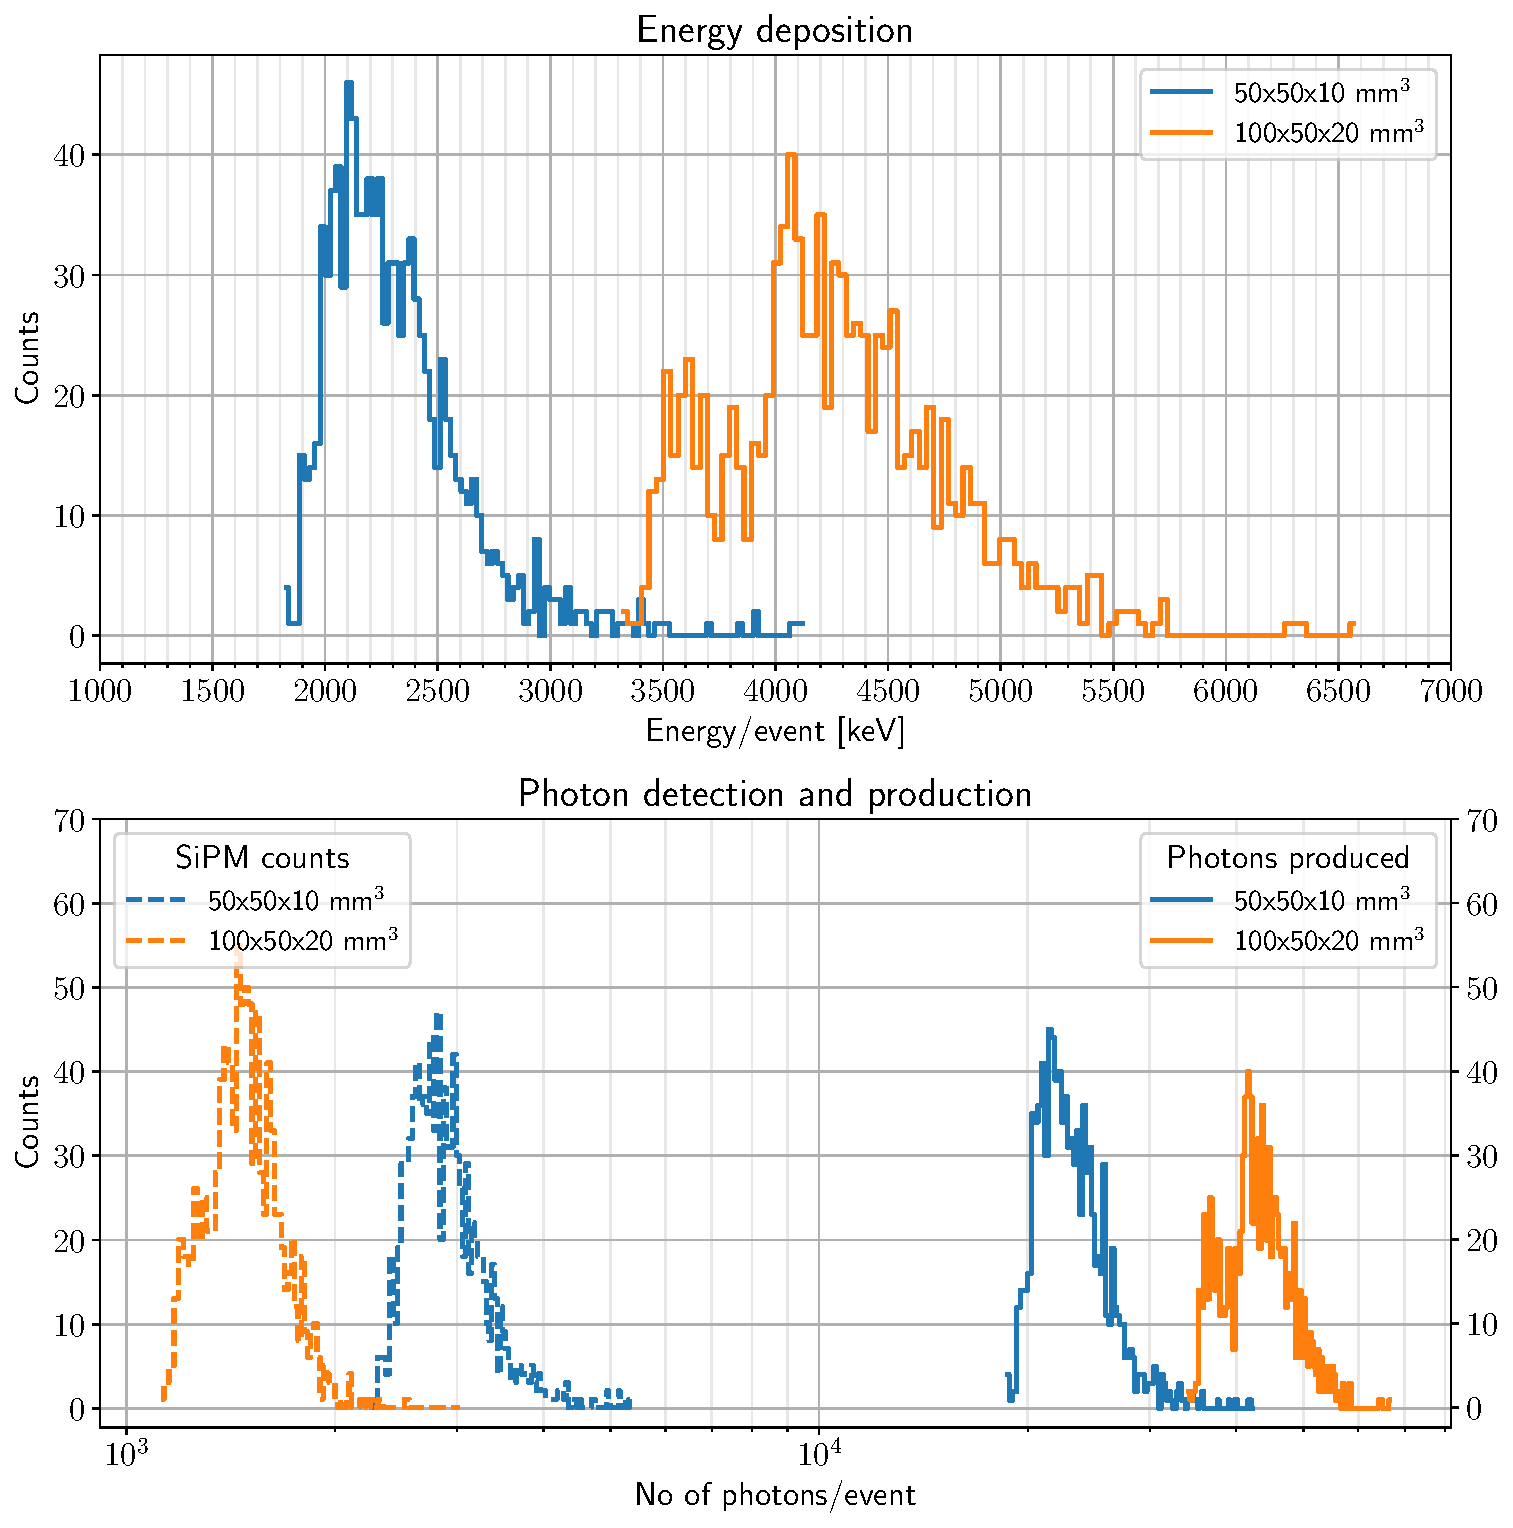
\includegraphics[width=.98\textwidth]{G4_simulations/PScint_photon_count/run0PScint.pdf}
  \caption{\label{fig:LYSO_PScint_phot_count}Energy deposition histograms for two sizes of plastics scintillator. The photon production inside the scintillator and photomultiplier photon counts are also compared for both sizes.}
\end{figure}

\subsection{SiPM placement}\label{sec:SiPM_placement}

The placement of the SiPM can be a factor to keep in mind while designing new CosmicWatch setups. Generally, the photomultiplier is located on the base of the scintillator as shown in Figure \ref{fig:geometry}, but it may be useful to place it on one of its sides as shown in Fig. \ref{fig:SiPM_side}.

\begin{figure}[H]
  \centering
  \begin{subfigure}[t]{0.48\textwidth}
    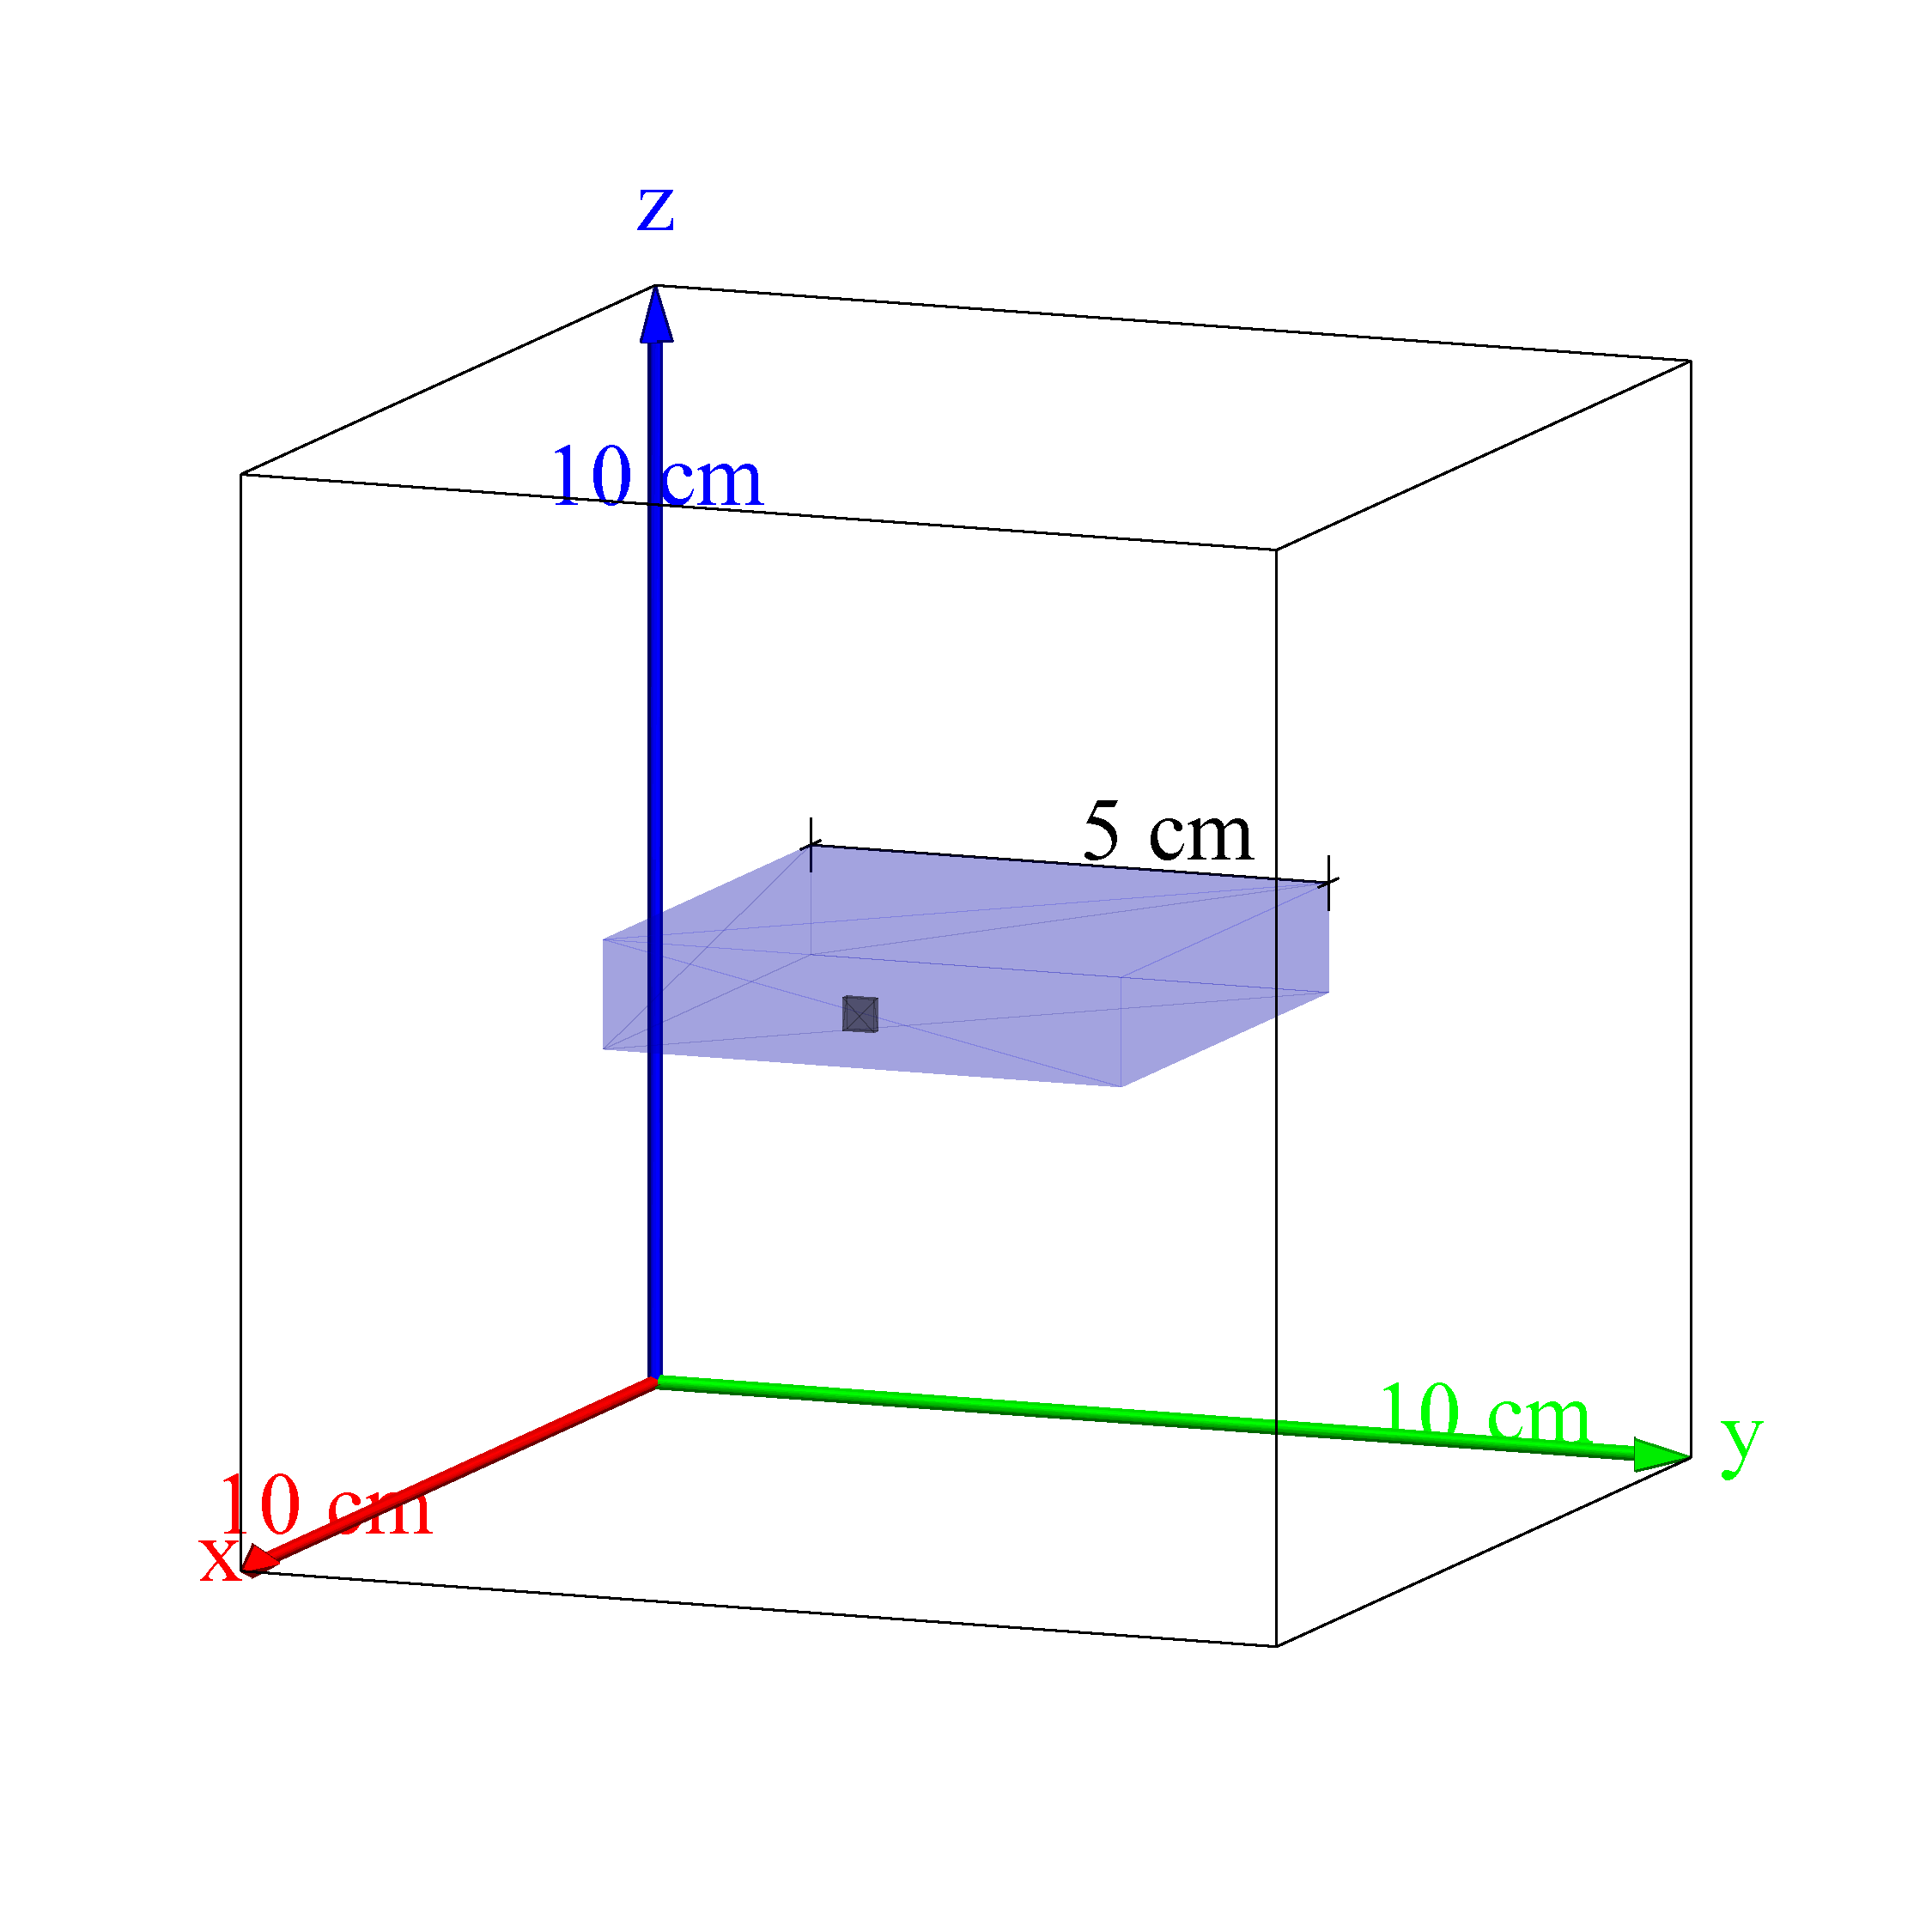
\includegraphics[width=\textwidth]{G4_simulations/SiPM_side_profile.pdf}
    \caption{\label{sfig:SiPM_side_profile}Diagonal view.}
  \end{subfigure}
  \hfill
  \begin{subfigure}[t]{0.48\textwidth}
    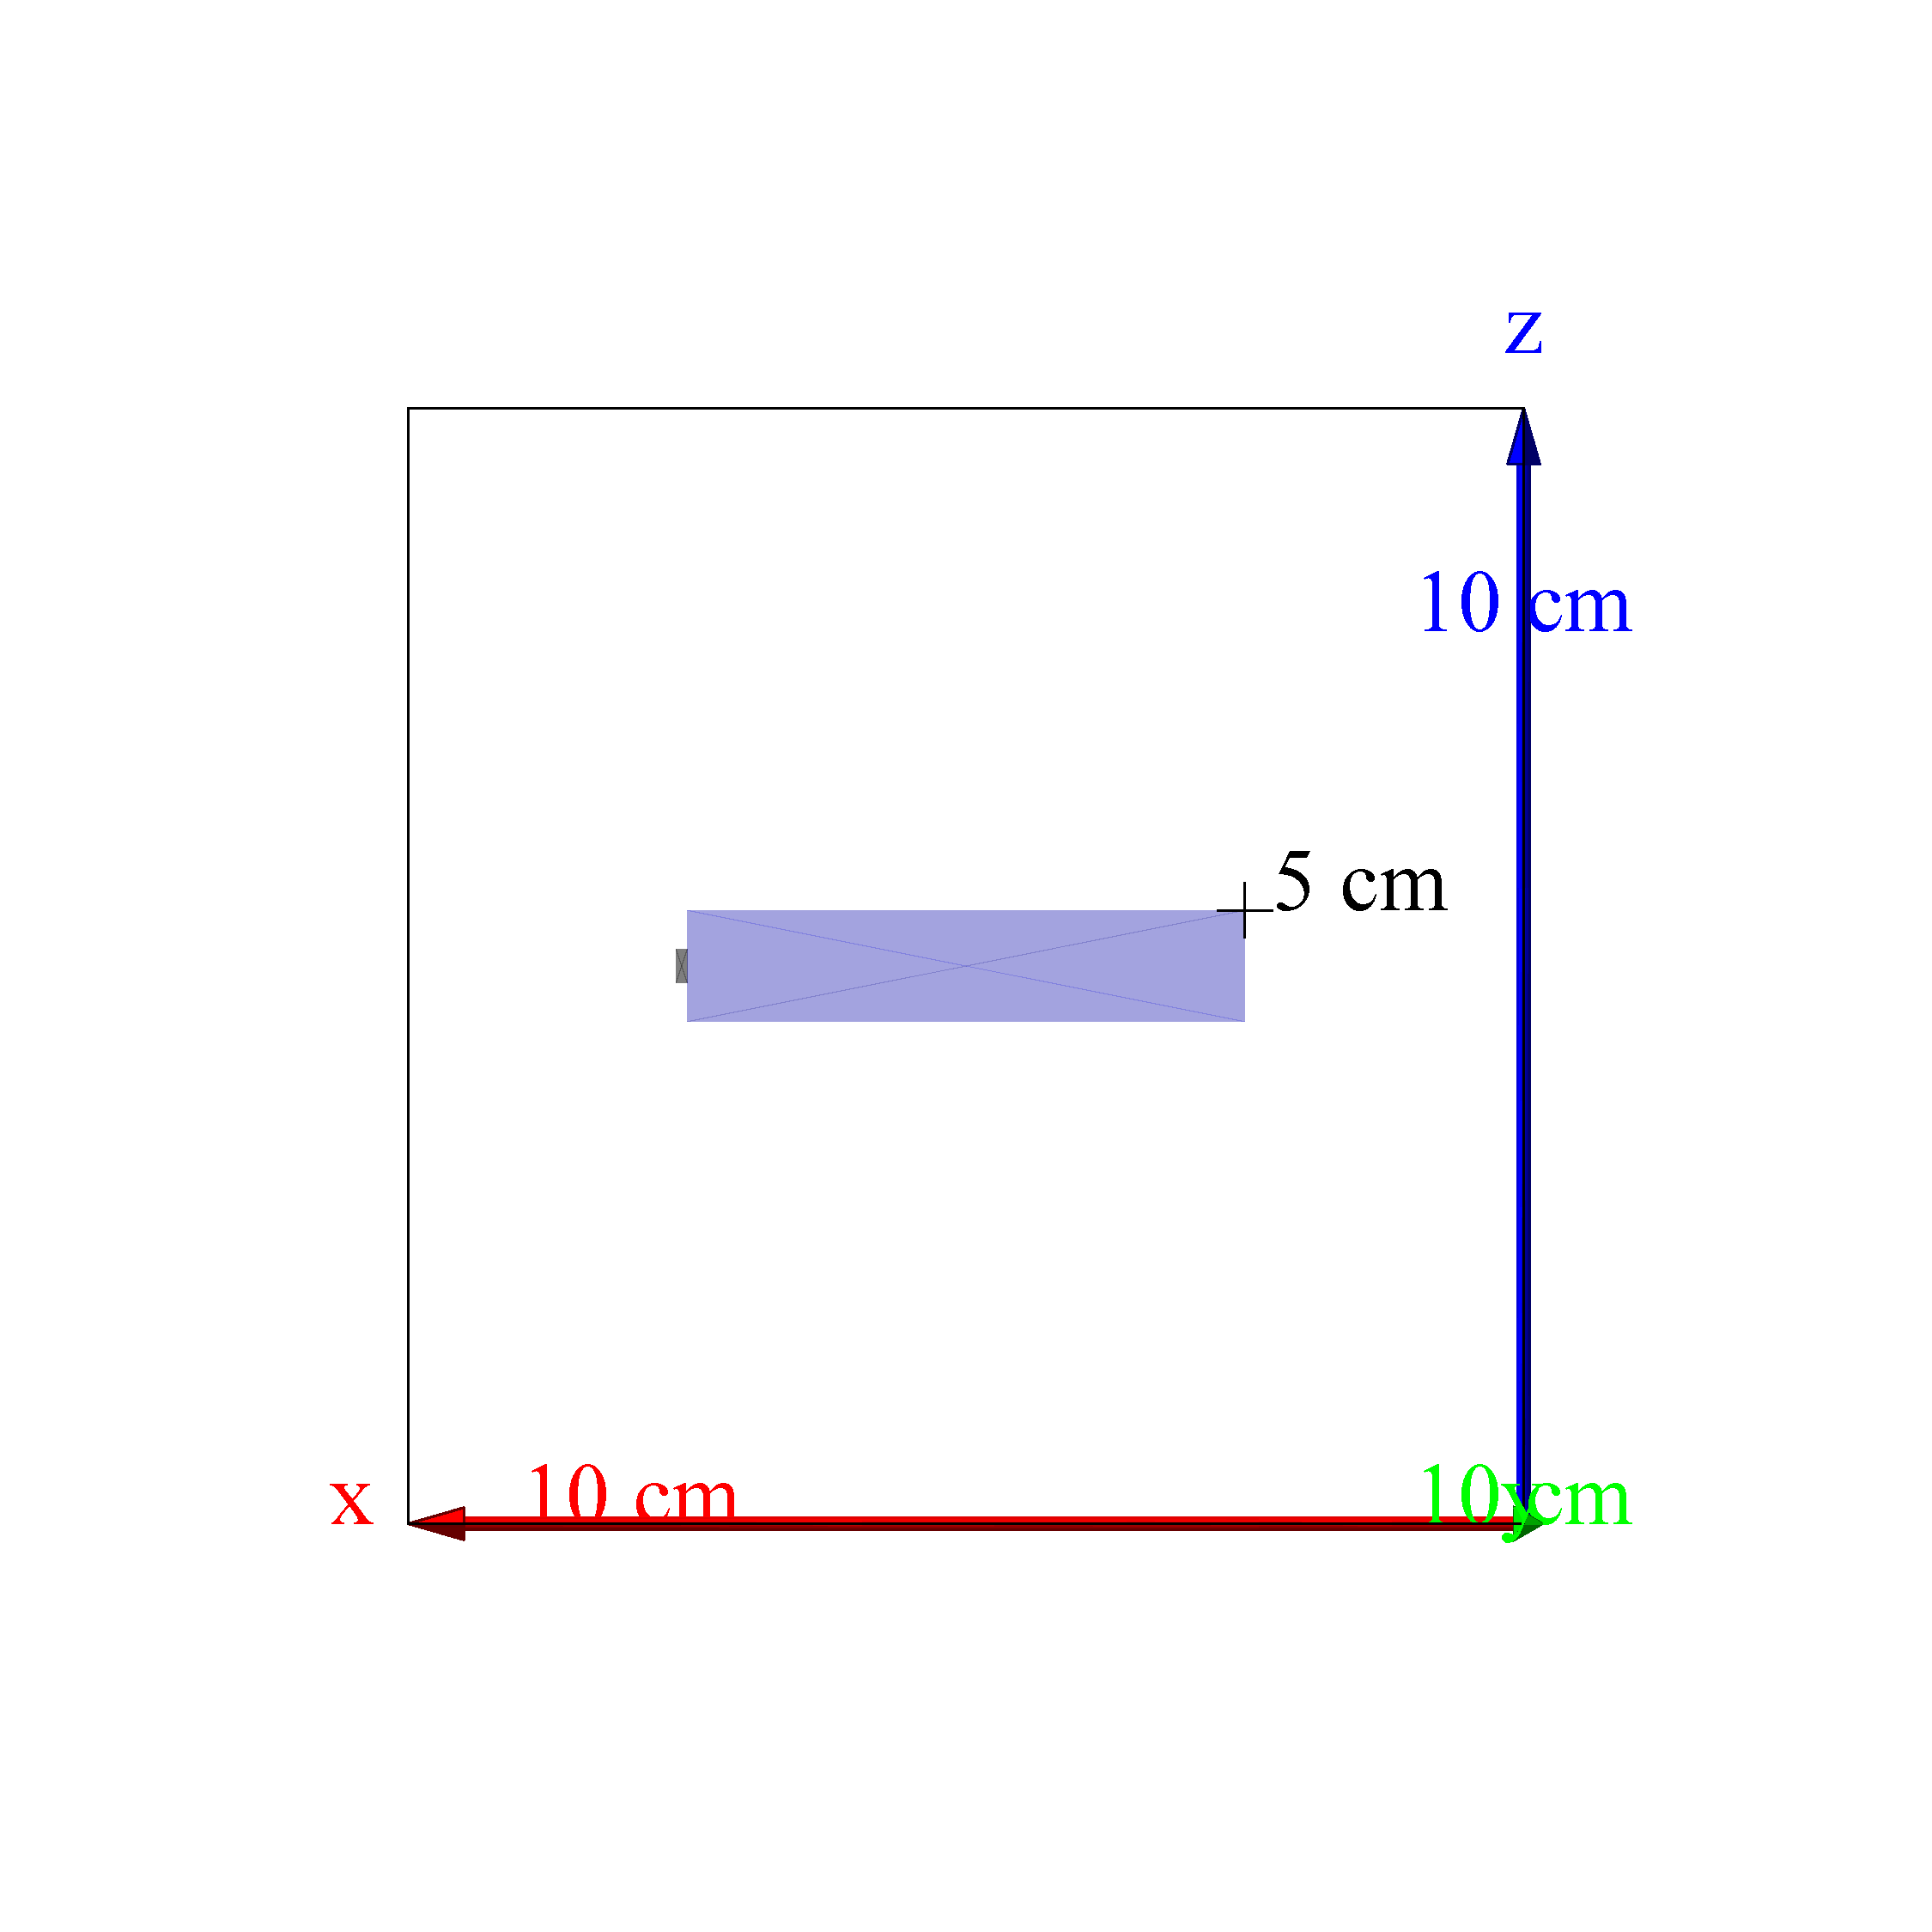
\includegraphics[width=\textwidth]{G4_simulations/SiPM_side_front.pdf}
    \caption{\label{sfig:SiPM_side_front}Side view.}
  \end{subfigure}
  \caption{\label{fig:SiPM_side}SiPM placed on the front face of the scintillator.}
\end{figure}

\begin{figure}[H]
    \centering
    \begin{subfigure}[t]{0.48\textwidth}
      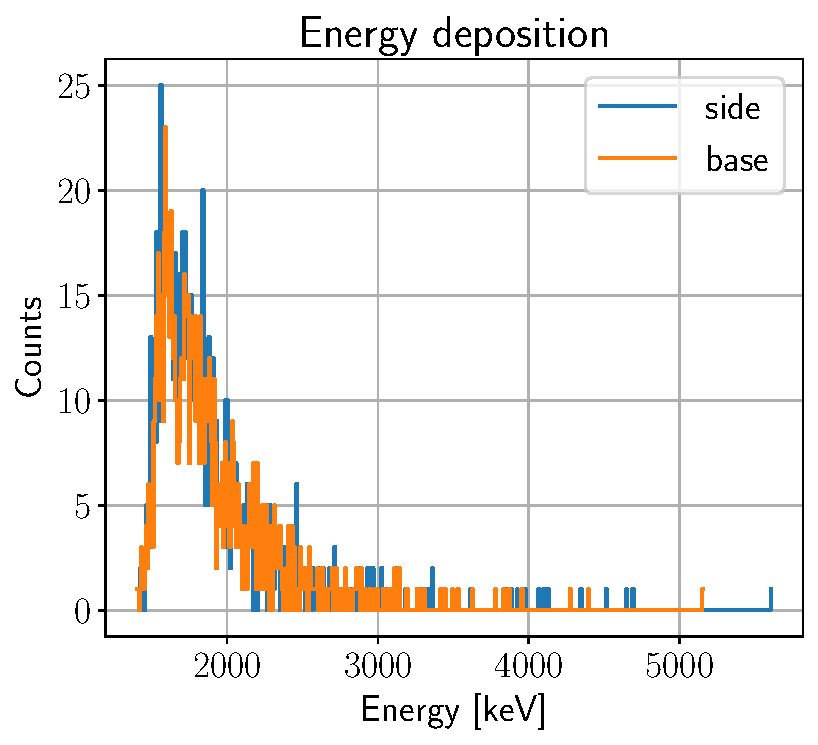
\includegraphics[width=\textwidth]{G4_simulations/run0_nt_Event_SiPM-placement_energy_spectra.pdf}
      \caption{\label{sfig:SiPM_place_edep}Energy deposition in the detector for different photomultiplier placements.}
    \end{subfigure}
    \hfill
    \begin{subfigure}[t]{0.48\textwidth}
      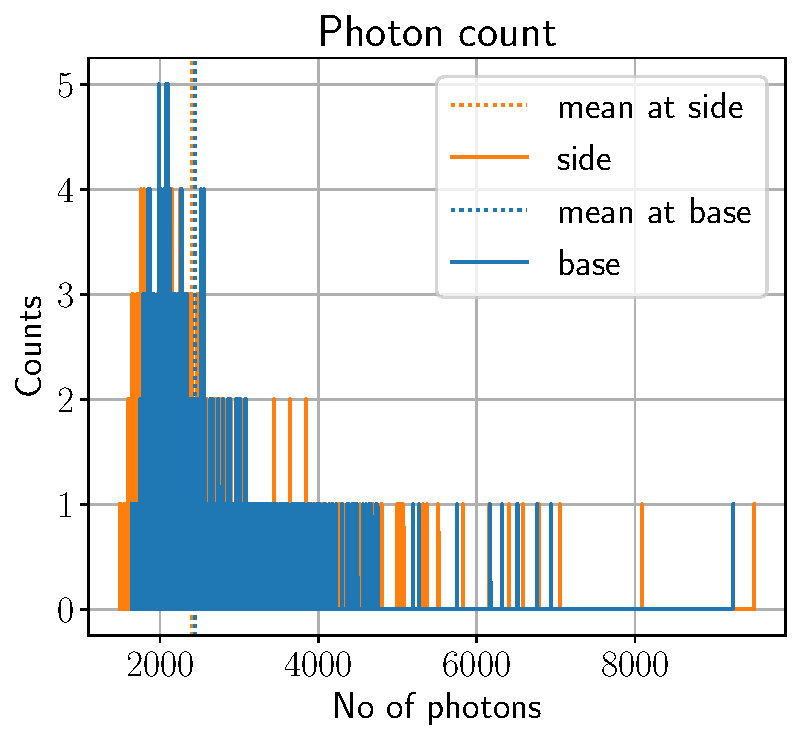
\includegraphics[width=\textwidth]{G4_simulations/run0_nt_Event_SiPM-placement_photon_count.pdf}
      \caption{\label{sfig:SiPM_place_pcount}SiPM photon count for both setups.}
    \end{subfigure}
    \caption{\label{fig:SiPM_place_results}}
\end{figure}

As expected, the energy deposition in the crystal and the number of optical photons produced do not depend on the SiPM placement. Surprisingly enough, however, it seems that the photon count is also not affected by this, meaning that the results obtained with both setups should be similar while using the specified scintillator size.

%\subsection{Scintillator sizes}\label{sec:Scint_size}

%The current architecture of CosmicWatch allows to use of variable scintillator sizes, the first versions of CosmicWatch used 5$\times$5$\times$1 \unit{\cm\cubed} scintillators, while the newer LYSO crystals are much smaller, Fig. \ref{fig:LYSO_crystals} shows some of the crystals used while testing the detector response. This simulation aims at understanding the effects of variable sizes in the final results.

%Figure \ref{sfig:scint_size_edep} shows that bigger scintillator sizes do result in greater energy recollections, however, as Figure \ref{sfig:scint_size_pcount} illustrates, the number of photons that reached the SiPM was on average greater for the $5\times5\times1$ \unit{\cm\cubed} setup. These figures then show that increased scintillator volumes may decrease photon recollection, which is ultimately the goal of the detector, to collect as many photons as possible in the photomultiplier to increase energy resolution.

%\begin{figure}[H]
%  \centering
%    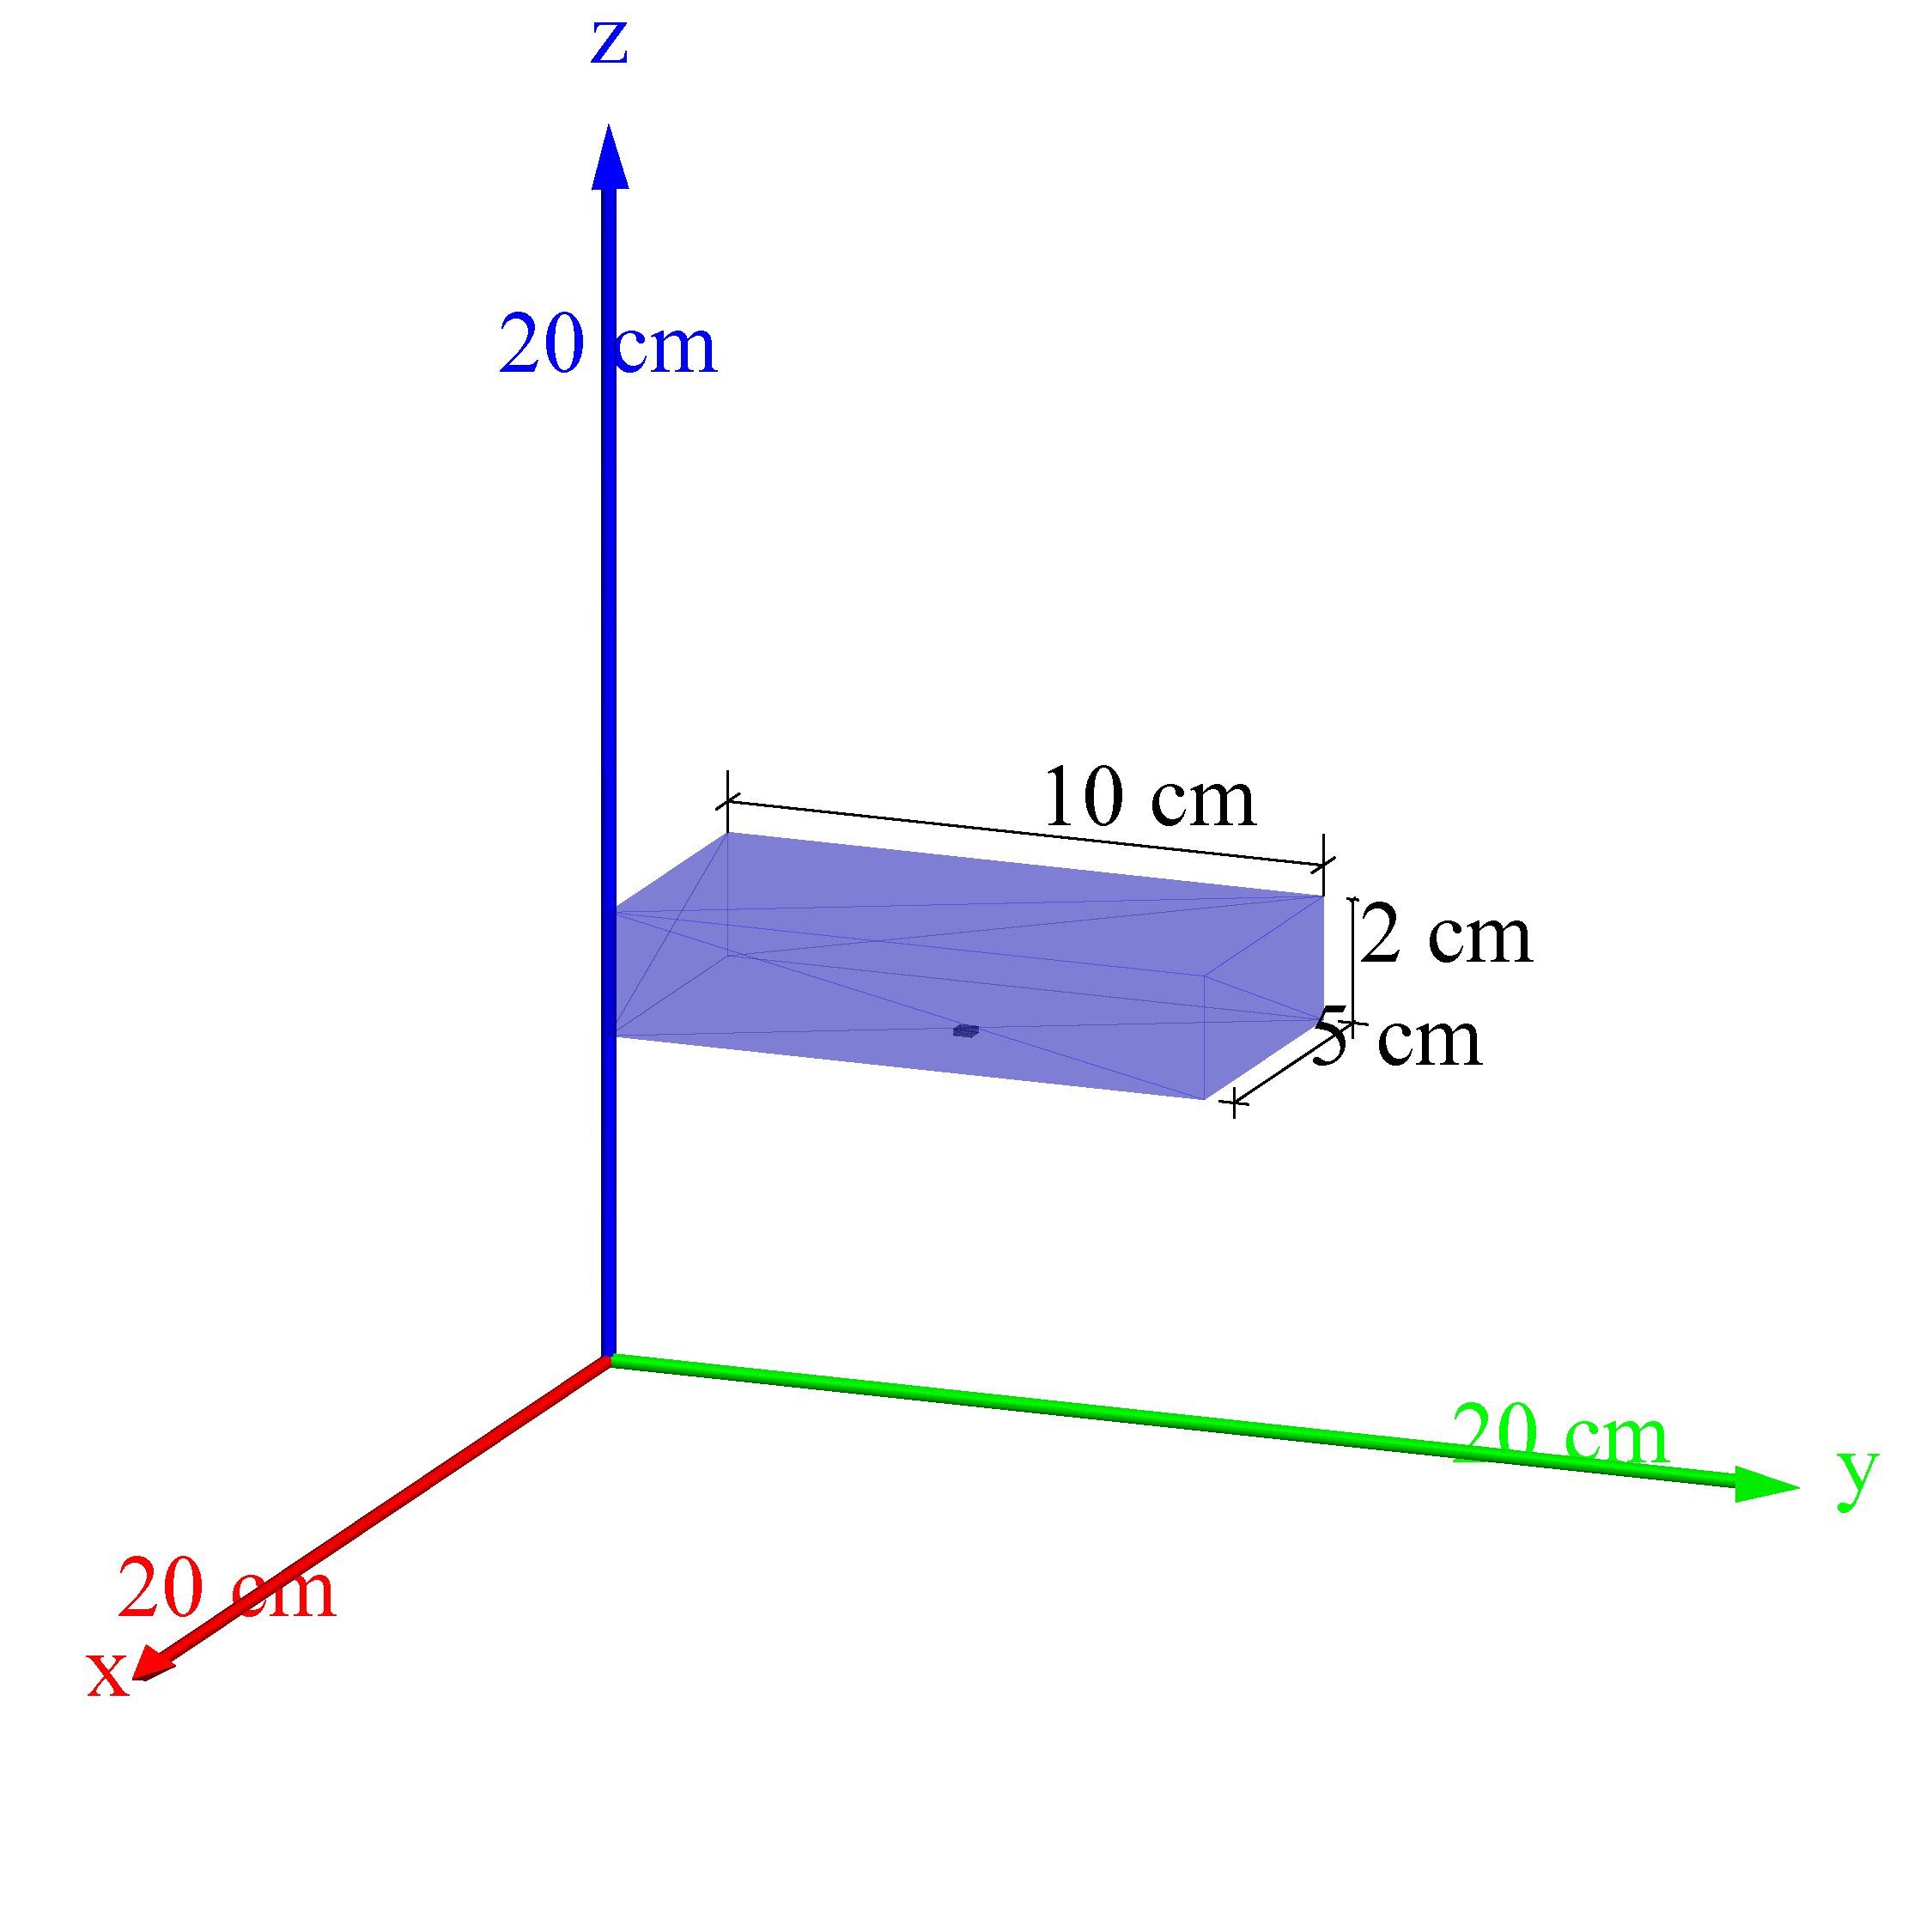
\includegraphics[width=0.47\textwidth]{G4_simulations/Scint_size_10_5_2.pdf}
%  \caption{\label{fig:Scint_10_5_2}Visualization of a bigger scintillator in the mother volume.}
%\end{figure}

%\begin{figure}[H]
%  \centering
%  \begin{subfigure}[t]{0.48\textwidth}
%    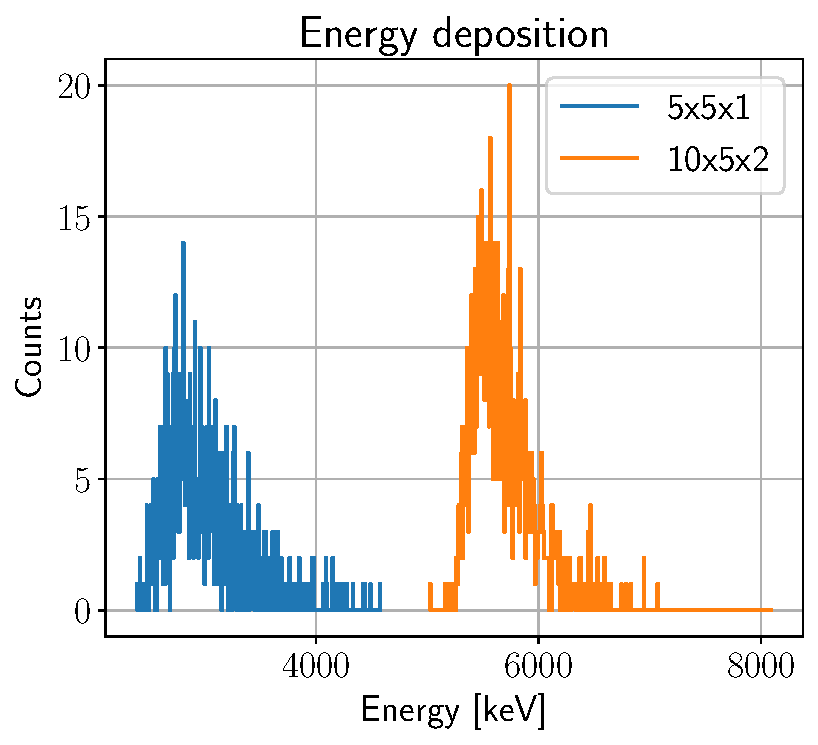
\includegraphics[width=\textwidth]{G4_simulations/run0_nt_Event_crystal-size_energy_spectra.pdf}
%    \caption{\label{sfig:scint_size_edep}Energy deposition in the detector for different scintillator sizes.}
%  \end{subfigure}
%  \hfill
%  \begin{subfigure}[t]{0.48\textwidth}
%    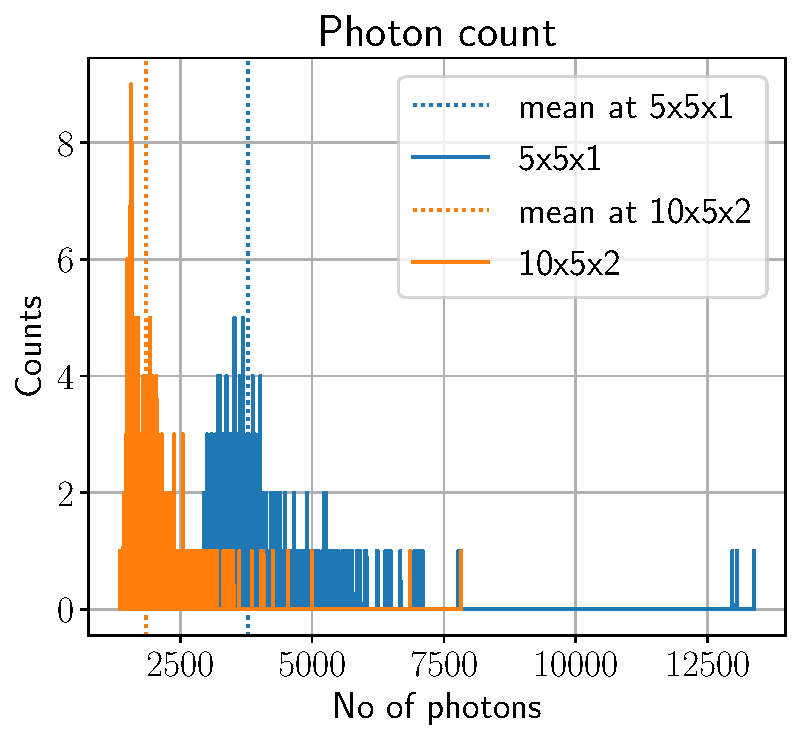
\includegraphics[width=\textwidth]{G4_simulations/run0_nt_Event_crystal-size_photon_count.pdf}
%    \caption{\label{sfig:scint_size_pcount}SiPM photon count for different scintillator sizes.}
%  \end{subfigure}
%  \caption{\label{fig:scint_size_results}The scintillator size can be easily modified inside the simulation by changing the values of \texttt{ScintXLen}, \texttt{ScintYLen}, and \texttt{ScintZLen} in \texttt{headers/construction.hh}, some suggested values are listed in the code.}
%\end{figure}

\subsection{Angular distributions}\label{sec:cos_squared}

With this simulation, we are trying to understand the detector response as a function of the zenith angle $\theta$, studying the energy deposition in the scintillating material and photon count in the SiPM depending on the trajectory of the particle once it enters the detector. As shown in Figure \ref{fig:ang_dist_cyl_event}, a spherical particle source was used to shoot particles from all directions toward the center of the scintillating crystal, however, this does not recreate the cosine squared law, as the particle source is isotropic, meaning that it does not have a preferred direction to shoot particles from. In order to recreate a cosine squared distribution the simulation data was multiplied by the function $\cos^2\theta$.

\begin{figure}[H]
  \centering
  \begin{subfigure}[t]{0.48\textwidth}
    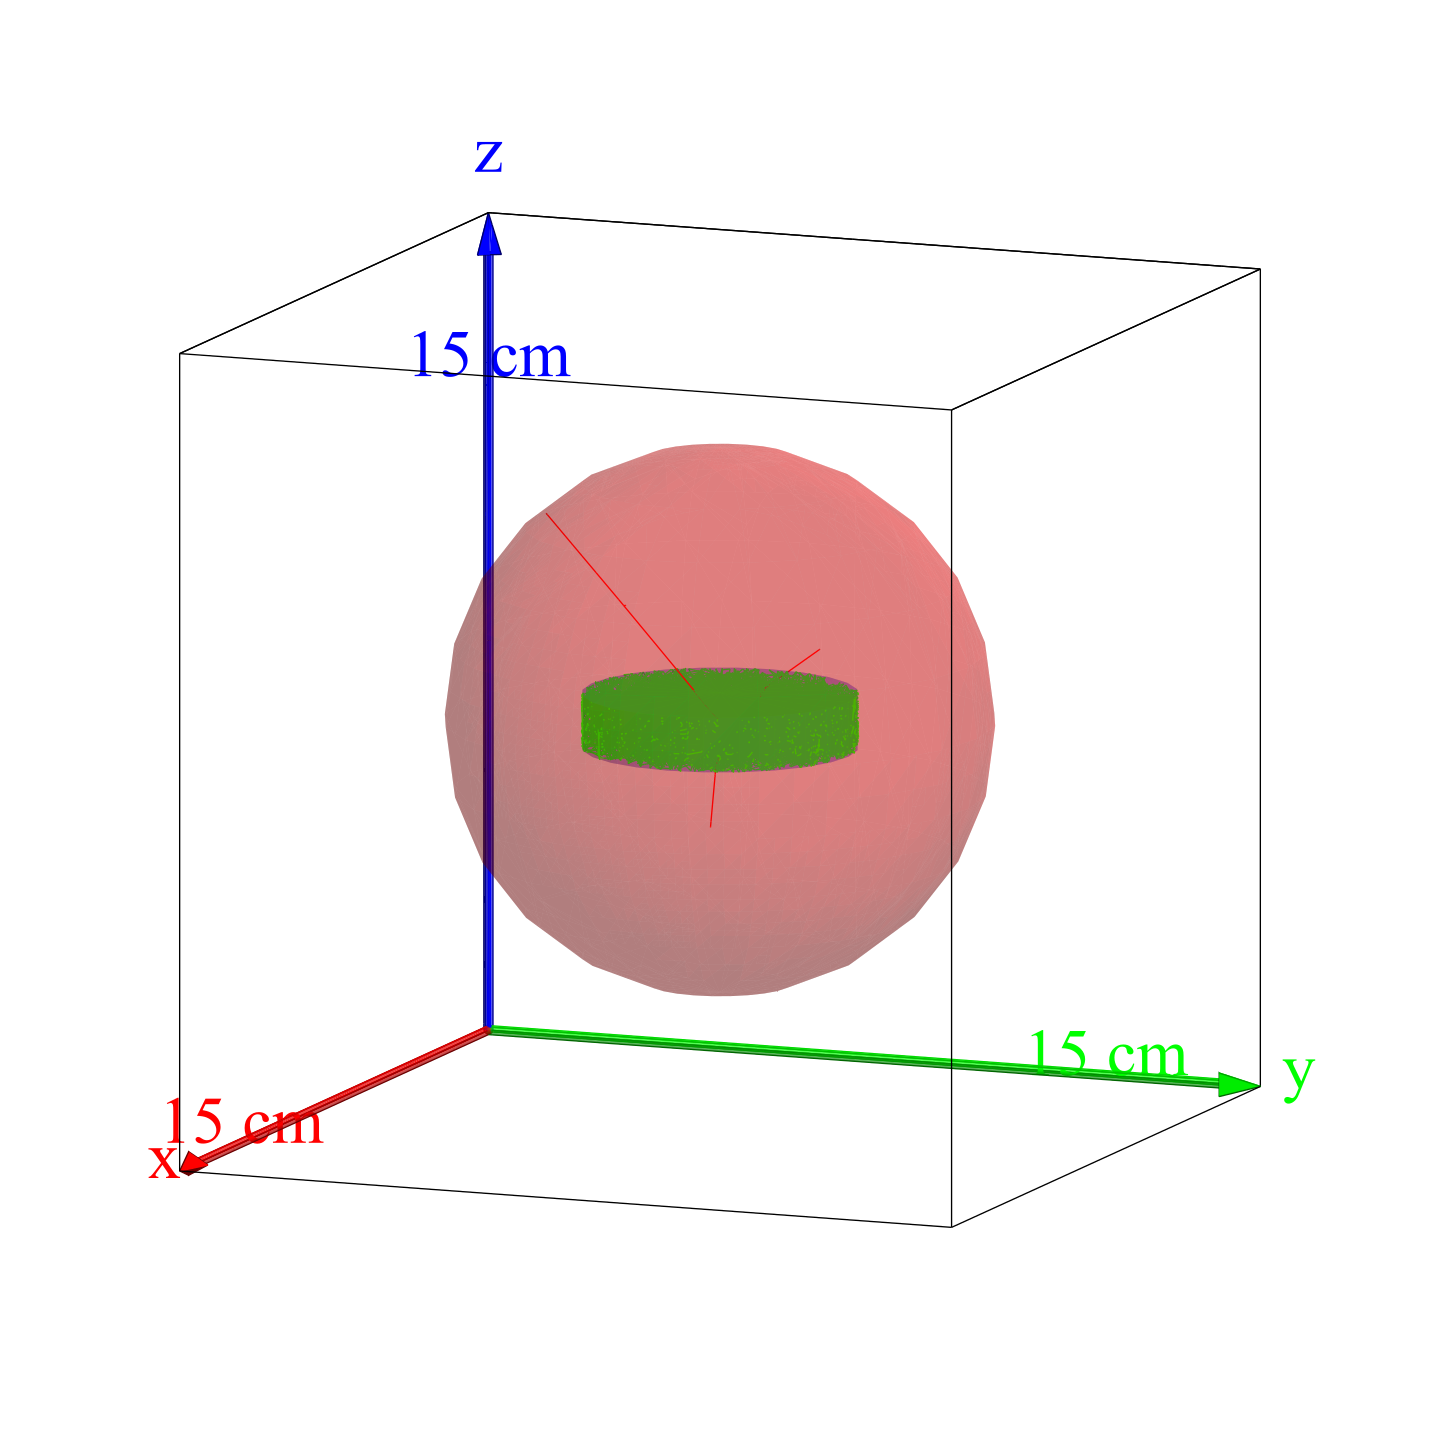
\includegraphics[width=\textwidth]{G4_simulations/ang_dist_cylinder_event_side.pdf}
    \caption{\label{sfig:ang_dist_cyl}}
  \end{subfigure}
  \hfill
  \begin{subfigure}[t]{0.48\textwidth}
    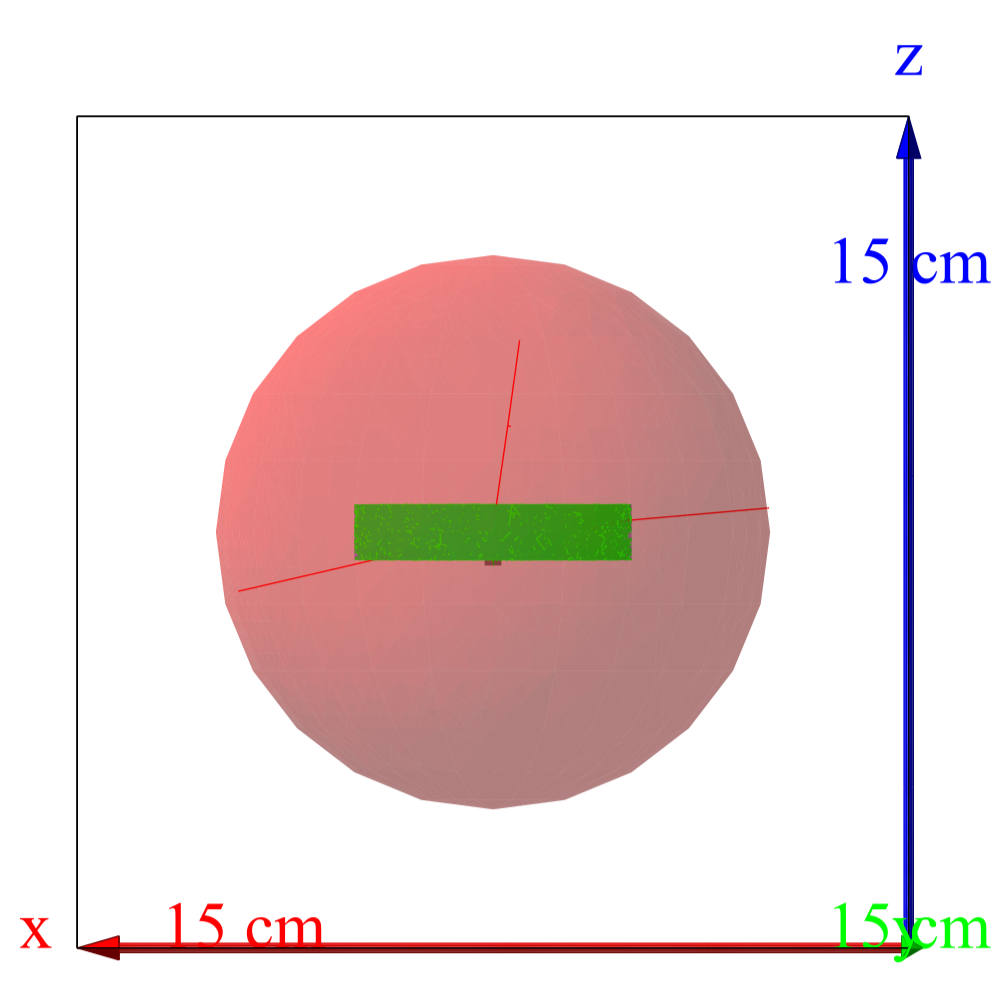
\includegraphics[width=\textwidth]{G4_simulations/ang_dist_cylinder_event.pdf}
    \caption{\label{sfig:ang_dist_cyl_side}}
  \end{subfigure}
  \caption{\label{fig:ang_dist_cyl_event}Spherical \gps~ shooting muons (\textcolor{red}{red} tracks) toward the center of a cylindrical plastic scintillator, the \textcolor{green}{green} tracks represent the optical photons produced from particle interactions.}
\end{figure}

As can be seen in Figure \ref{sfig:ang_dist_cyl_side}, muons traveling directly downward have less scintillating material to go through compared to those traveling horizontally, this means that greater zenith angles should result in greater energy depositions, which agrees with the data shown in Figures \ref{sfig:ang_edep} and \subref{sfig:ang_edep_cylinder}. In Figure \ref{sfig:ang_pcount} however, the photon counts first decrease to a minimum at around 30$^\circ$ before steadily increasing until 90$^\circ$. Based on what we learned in section \ref{sec:collected_produced} about scintillator sizes, and keeping in mind the detector geometry, one could expect a minimum photon count at the angle where the photons have to travel the greatest distance within the scintillator, which in this case corresponds to the scintillator edges and corners, ranging between 78.69 and 81.95 degrees for a $5\times5\times1$ \unit{\cm\cubed} scintillator. In order to attenuate any possible polar dependencies, the scintillator geometry was changed to a cylinder as shown in Figure \ref{fig:ang_dist_cyl_event}. This however, does not seem to correlate with the presence of a minimum in photon count at 30$^\circ$, as can be seen in Figure \ref{sfig:ang_pcount_cylinder}. The cause of this feature is yet to be explained.

\begin{figure}[H]
  \centering
  \begin{subfigure}[t]{0.48\textwidth}
    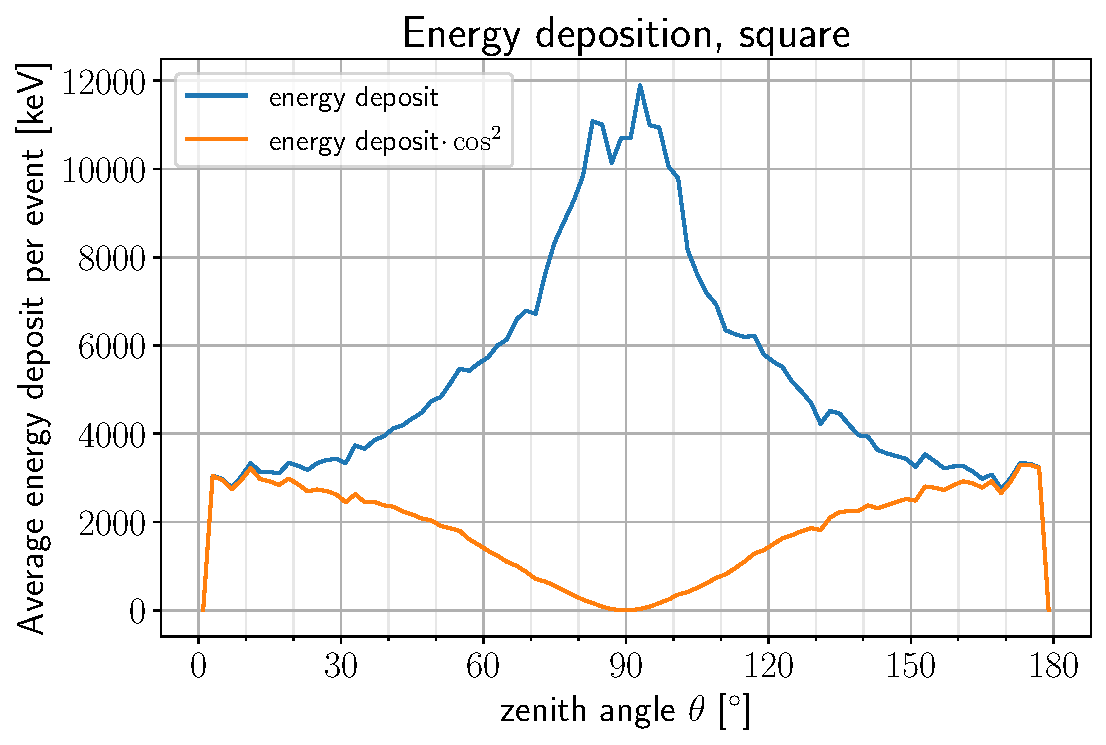
\includegraphics[width=\textwidth]{G4_simulations/run0-ang_dis_nt_Event_energy_spectra.pdf}
    \caption{\label{sfig:ang_edep}Energy deposition in the detector as a function of zenith angle.}
  \end{subfigure}
  \hfill
  \begin{subfigure}[t]{0.48\textwidth}
    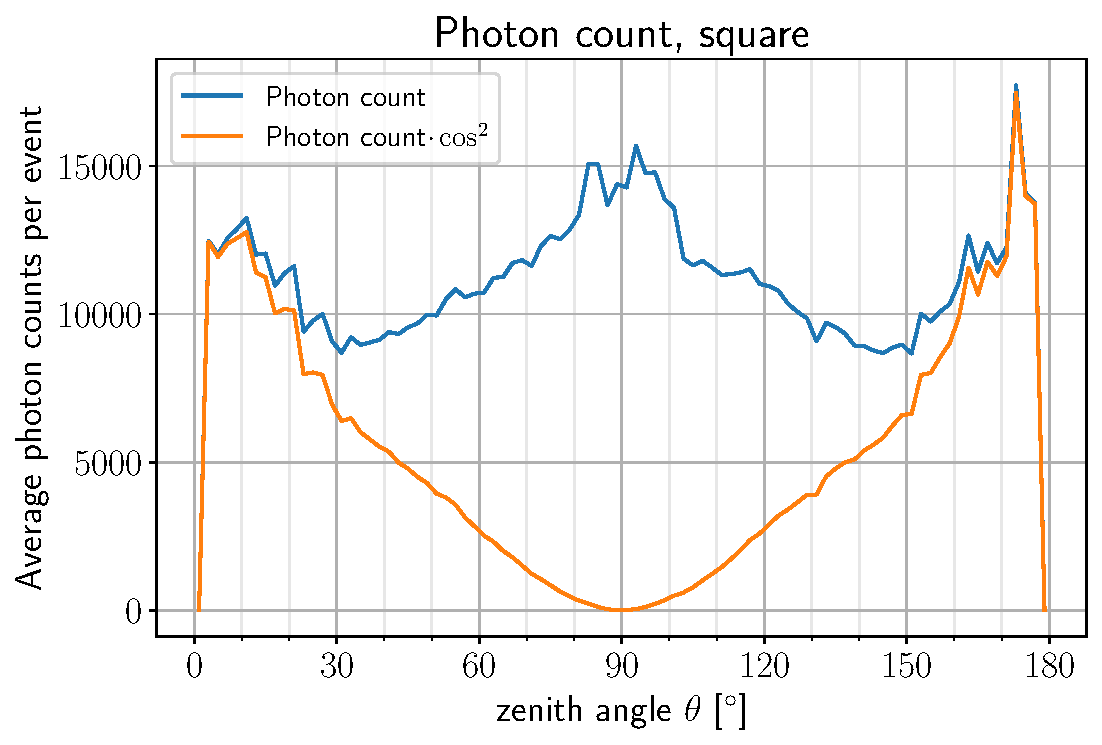
\includegraphics[width=\textwidth]{G4_simulations/run0-ang_dis_nt_Event_photon_count.pdf}
    \caption{\label{sfig:ang_pcount}SiPM photon as a function of zenith angle.}
  \end{subfigure}
  \medskip
  \begin{subfigure}[t]{0.48\textwidth}
    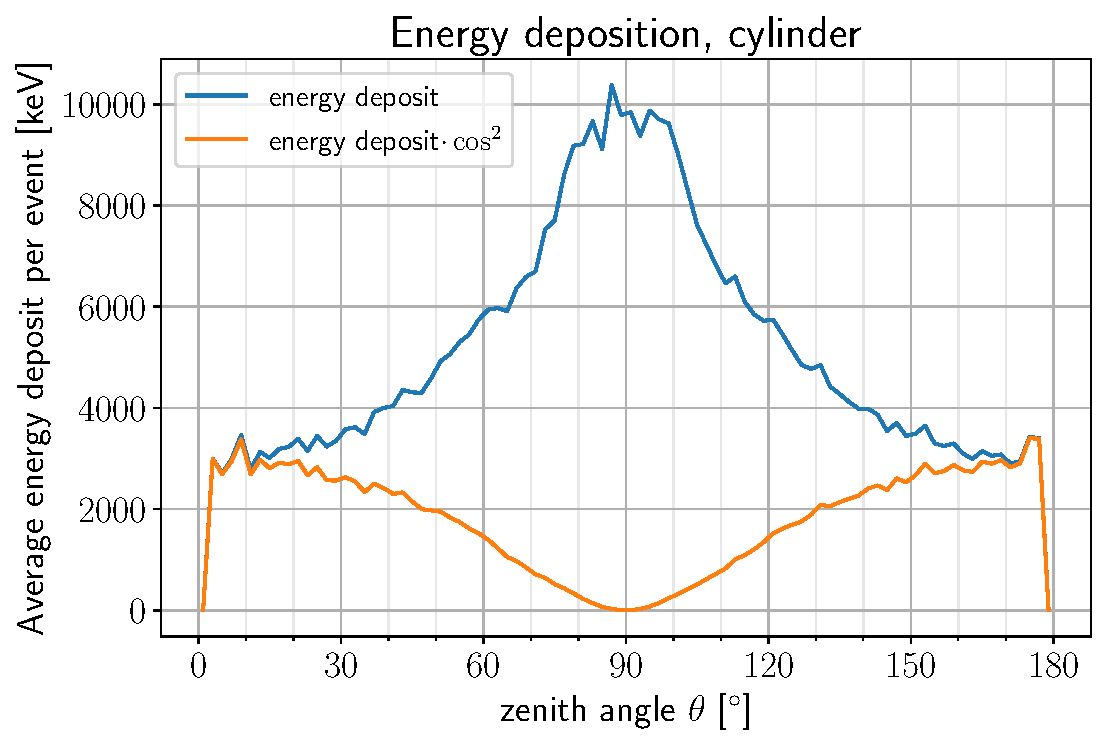
\includegraphics[width=\textwidth]{G4_simulations/test_nt_Event_energy_spectra.pdf}
    \caption{\label{sfig:ang_edep_cylinder}Energy deposition in the detector as a function of zenith angle with a cylindrical scintillator.}
  \end{subfigure}
  \hfill
  \begin{subfigure}[t]{0.48\textwidth}
    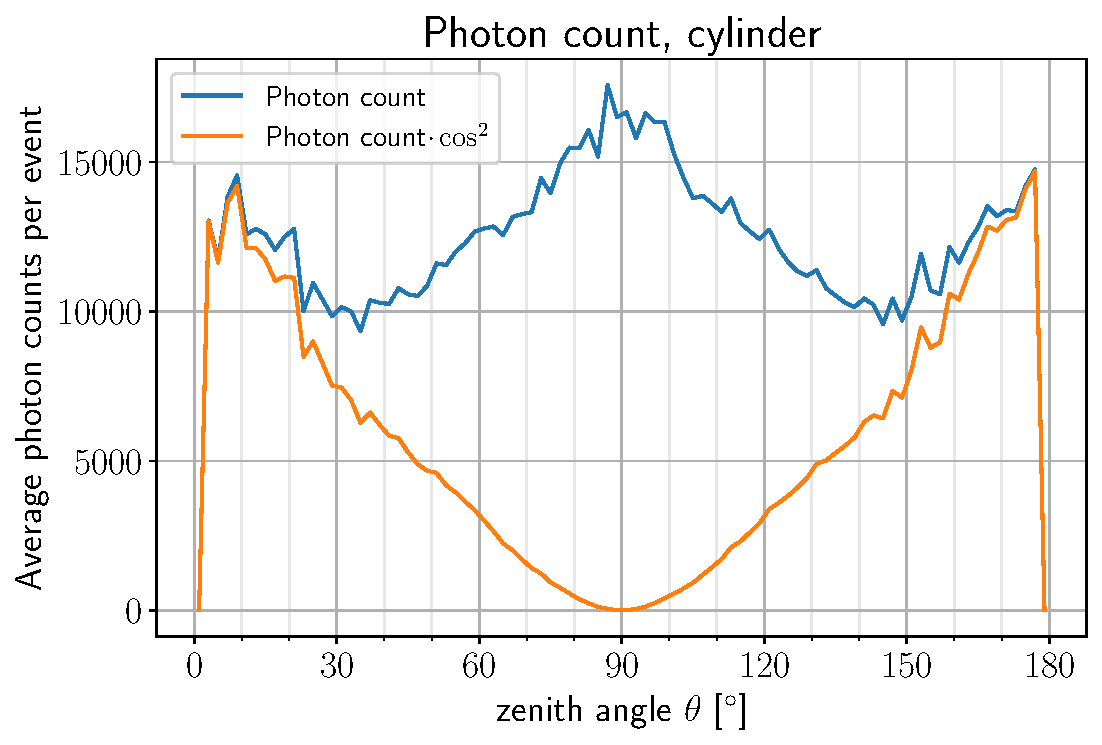
\includegraphics[width=\textwidth]{G4_simulations/test_nt_Event_photon_count.pdf}
    \caption{\label{sfig:ang_pcount_cylinder}SiPM photon as a function of zenith angle with a cylindrical scintillator.}
  \end{subfigure}
  \caption{\label{fig:ang_results}Data in blue is the raw output of the simulation while shooting muons directly toward the center of the scintillator. Data in orange is the normalization of the simulation output using a cosine squared law.}
\end{figure}

\subsection{Simulated Spectra}\label{sec:simulated_spectra}

In order to showcase some of the differences between LYSO and plastic scintillators we have included some simulation results for both LYSO and \texttt{Polyvinyltoluene}. The analysis presented below corresponds to ten thousand events where the \gps shoots 662 \unit{\kilo\eV} gamma-rays.

As discussed in Section \ref{sec:self_radiation}, LYSO crystals contain $^{176}$Lu, a naturally occurring radioactive isotope emitting $\beta$ radiation which can be absorbed by the crystal, this results in a constant background, this feature, however, has not yet been included in the simulation and is part of our future work.

Contrary to \texttt{G4\_PLASTIC\_SC\_VINYLTOLUENE} and \texttt{G4\_Air}, there is no \texttt{G4\_LYSO}, which in this case is needed to produce gamma-spectra since this plastic scintillator does not produce enough photoelectric events to obtain something similar to the spectra shown in Section \ref{sec:gammas_in_the_detector}. Luckily Geant4 allows to create materials by adding individual elements with their respective percentage in the compound. Table \ref{tab:LYSO_composition} shows the specific percentages for all elements that make up a LYSO. In order to add Cerium doping one can create a new material made of two parts, LYSO and Ce, in this case, one would use the doping percentage to calculate the amount of LYSO in the new compound. It hasn't been possible to find the specific amount of Ce doping in Luxium's LYSO, there are however some publications that reference doping below 1.\% for Saint-Gobain samples \cite{Ce_doping,Ce_dopping_2}\footnote{Luxium and Saint-Gobain's LYSOs are essentially the same since Luxium acquired the scintillation and photonic crystals business of Saint-Gobain.}. All material definitions can be found under the function \texttt{DefineMaterials} of \texttt{MyDetectorConstruction} class in \texttt{source/construction.cc}.

\begin{table}[H]
  \caption{Atomic mass and composition percentage for all elements in the nominal composition Lu$_{1.8}$Y$_{0.2}$SiO$_5$:Ce.}
  \centering
  \begin{tabular}{ c c c c c}
    \midrule
     & Lu & Y & Si & O \\
    \midrule
    atomic mass [amu] & 174.967 & 88.906 & 28.086 & 15.999 \\
    \% & 71.447 & 4.034 & 6.371 & 18.148 \\
    \bottomrule
  \end{tabular}
  \label{tab:LYSO_composition}
\end{table}

Figure \ref{fig:LYSO_edep} shows the obtained energy spectra for the three crystal sizes shown in Figure \ref{fig:LYSO_crystals} while shooting monoenergetic 662 \unit{\kilo\eV} gamma rays. In this case, the photopeak is almost a Dirac delta since this is the Monte Carlo truth, no noise is introduced while counting the energy deposition. It is interesting to see that the counts start to drop after the Compton edge at 478 \unit{\kilo\eV}, there should be however zero counts between $E_C$ and the photopeak. Figure \ref{fig:LYSO_edep} also demonstrates one of the advantages of LYSO over plastic scintillators, the high density of LYSO increases the probability of photoelectric interactions, while BC404 lets gammas through more often (0 energy deposition).

The count of photons produced per event (Fig. \ref{fig:LYSO_ScintPhotons}) seems to uniformly increase with crystal size just like the energy deposition, this is expected since bigger crystals produce higher travel paths for the gammas, increasing the chance of interactions and therefore photon production. Here we also see something close to a Dirac delta above twenty thousand, this is due to the \texttt{RESOLUTIONSCALE} value $(=0.0)$ in the scintillator's \texttt{G4MaterialPropertiesTable}, this resolution determines the standard deviation of the Gaussian function used to calculate the number of produced photons\footnote{A Poisson distribution is used if the expected number of photons $(E_{dep}\cdot L_{yield})$ is less or equal to 10.}, given by having $\sigma=\texttt{RESOLUTIONSCALE}~\sqrt{E_{dep}\cdot L_{yield}}$. The \texttt{SCINTILLATIONYIELD} values in the simulation are those shown in Table. \ref{tab:scintillators}, this explains the overwhelming number of photons produced by LYSO compared to the plastic scintillator. It is also notable that for bigger sizes LYSO tends to let fewer gammas pass through it without interacting (zero photons produced).

\begin{figure}
  \centering
  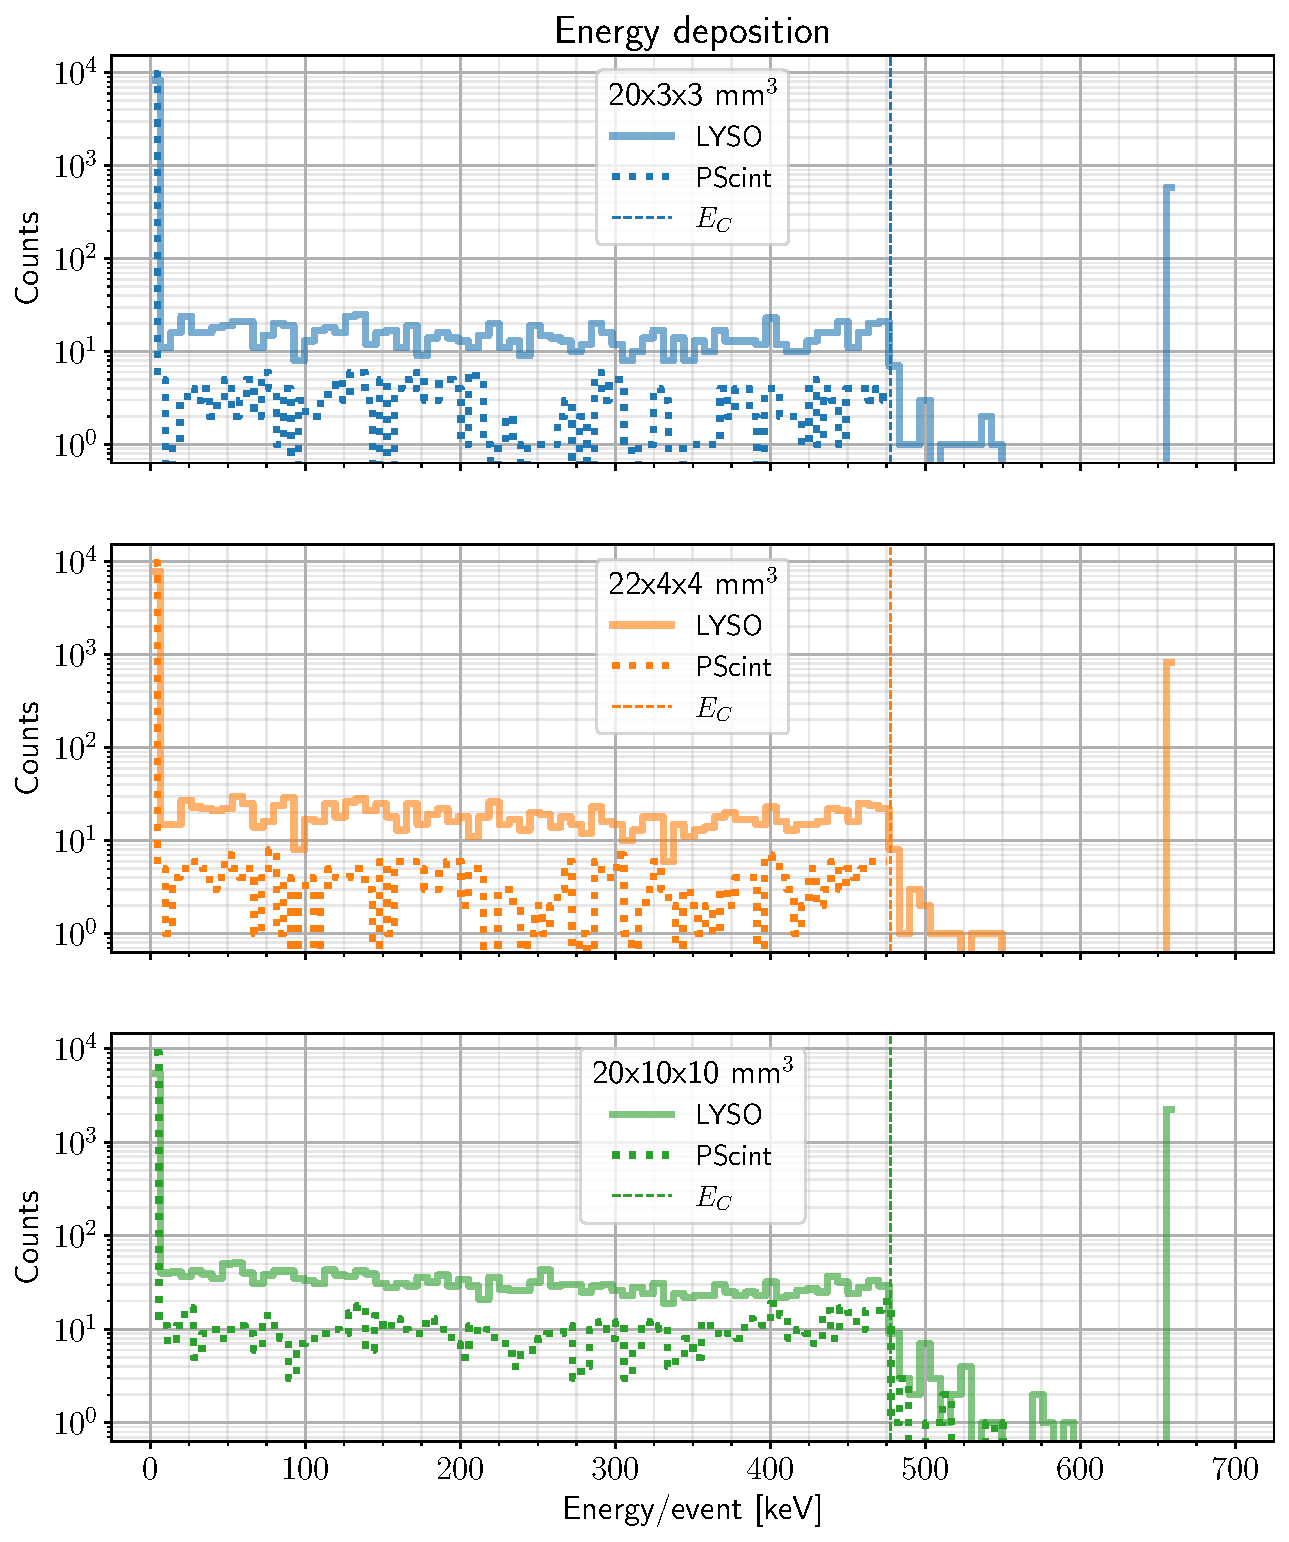
\includegraphics[width=.98\textwidth]{G4_simulations/gammas/run0energy_spectra.pdf}
  \caption{\label{fig:LYSO_edep}Energy deposition per event in LYSO and plastic scintillator using three different crystal sizes. In this case the \gps~ shoots 662 \unit{\kilo\eV} gamma-rays.}
\end{figure}

\begin{figure}
  \centering
  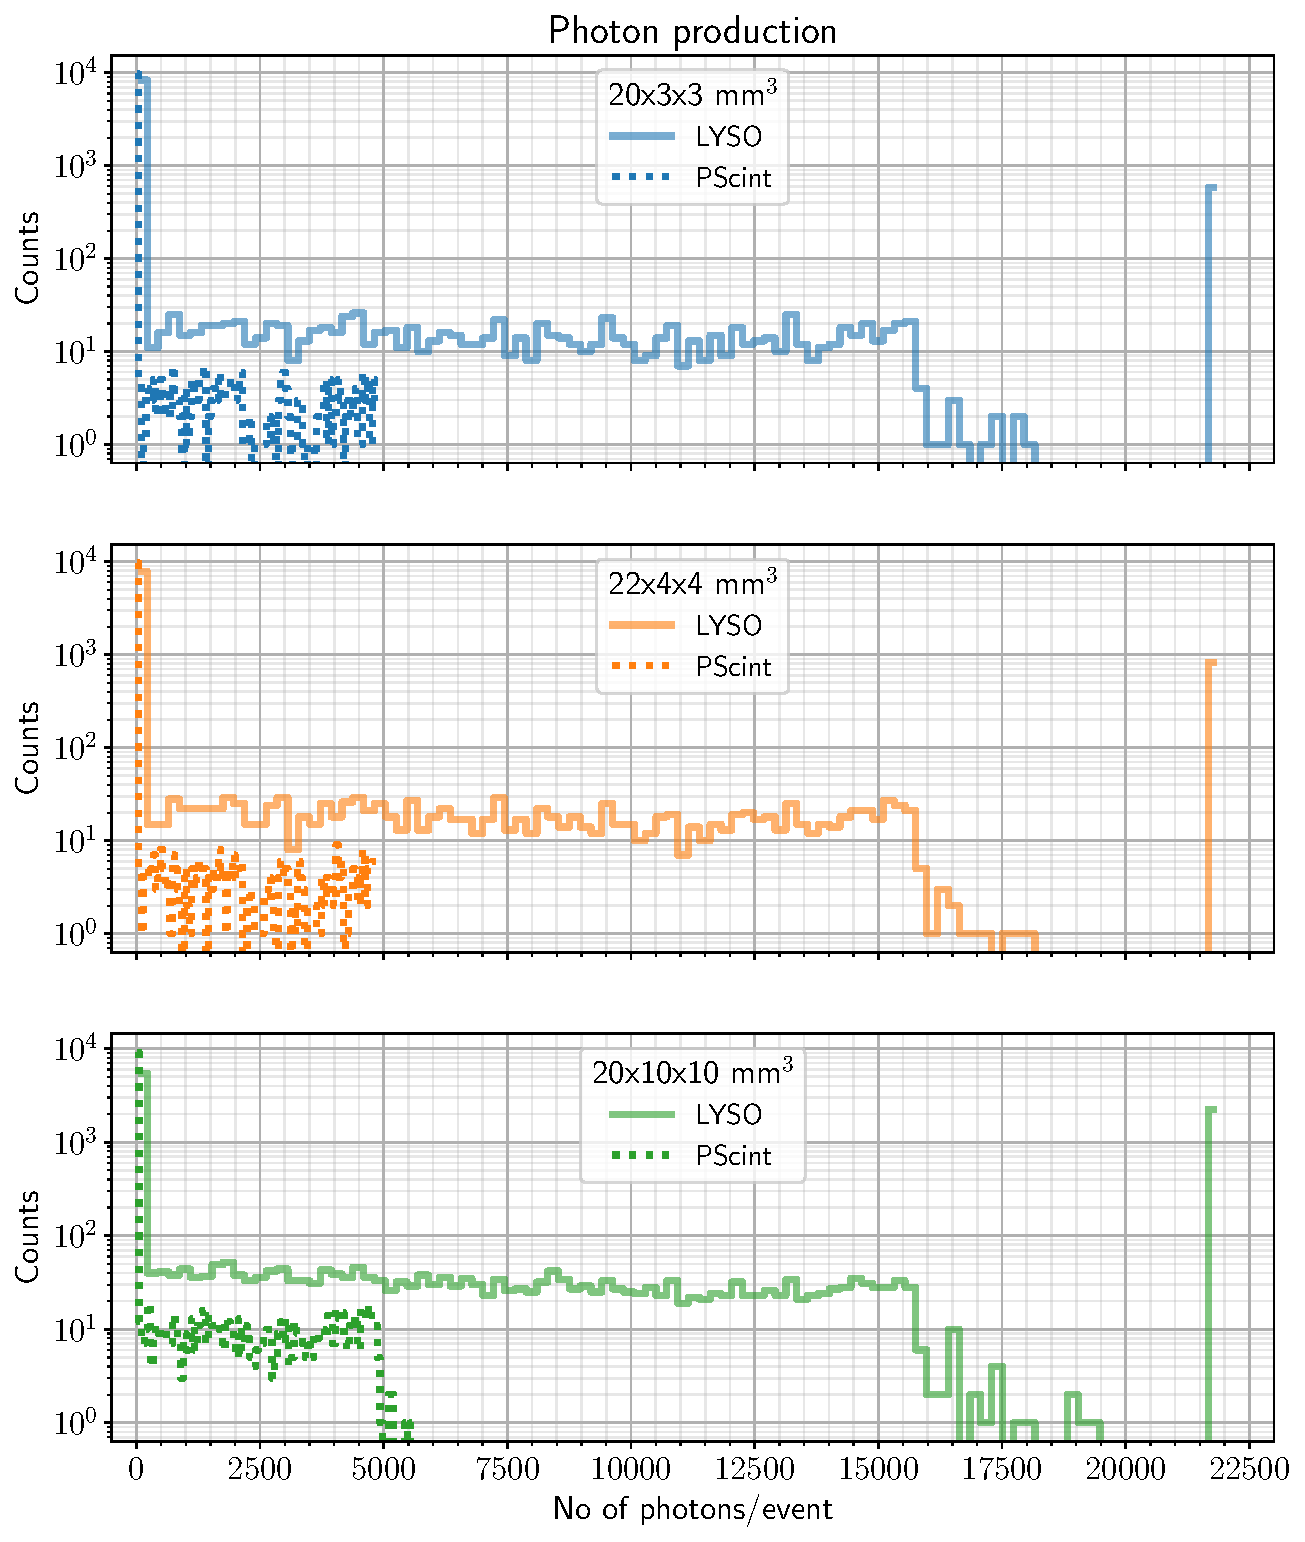
\includegraphics[width=.98\textwidth]{G4_simulations/gammas/run0ScintPhotons.pdf}
  \caption{\label{fig:LYSO_ScintPhotons}Optical photon production per event in LYSO and plastic scintillator, showing three different crystal sizes. In this case the \gps~ shoots 662 \unit{\kilo\eV} gamma-rays.}
\end{figure}

\begin{figure}
  \centering
  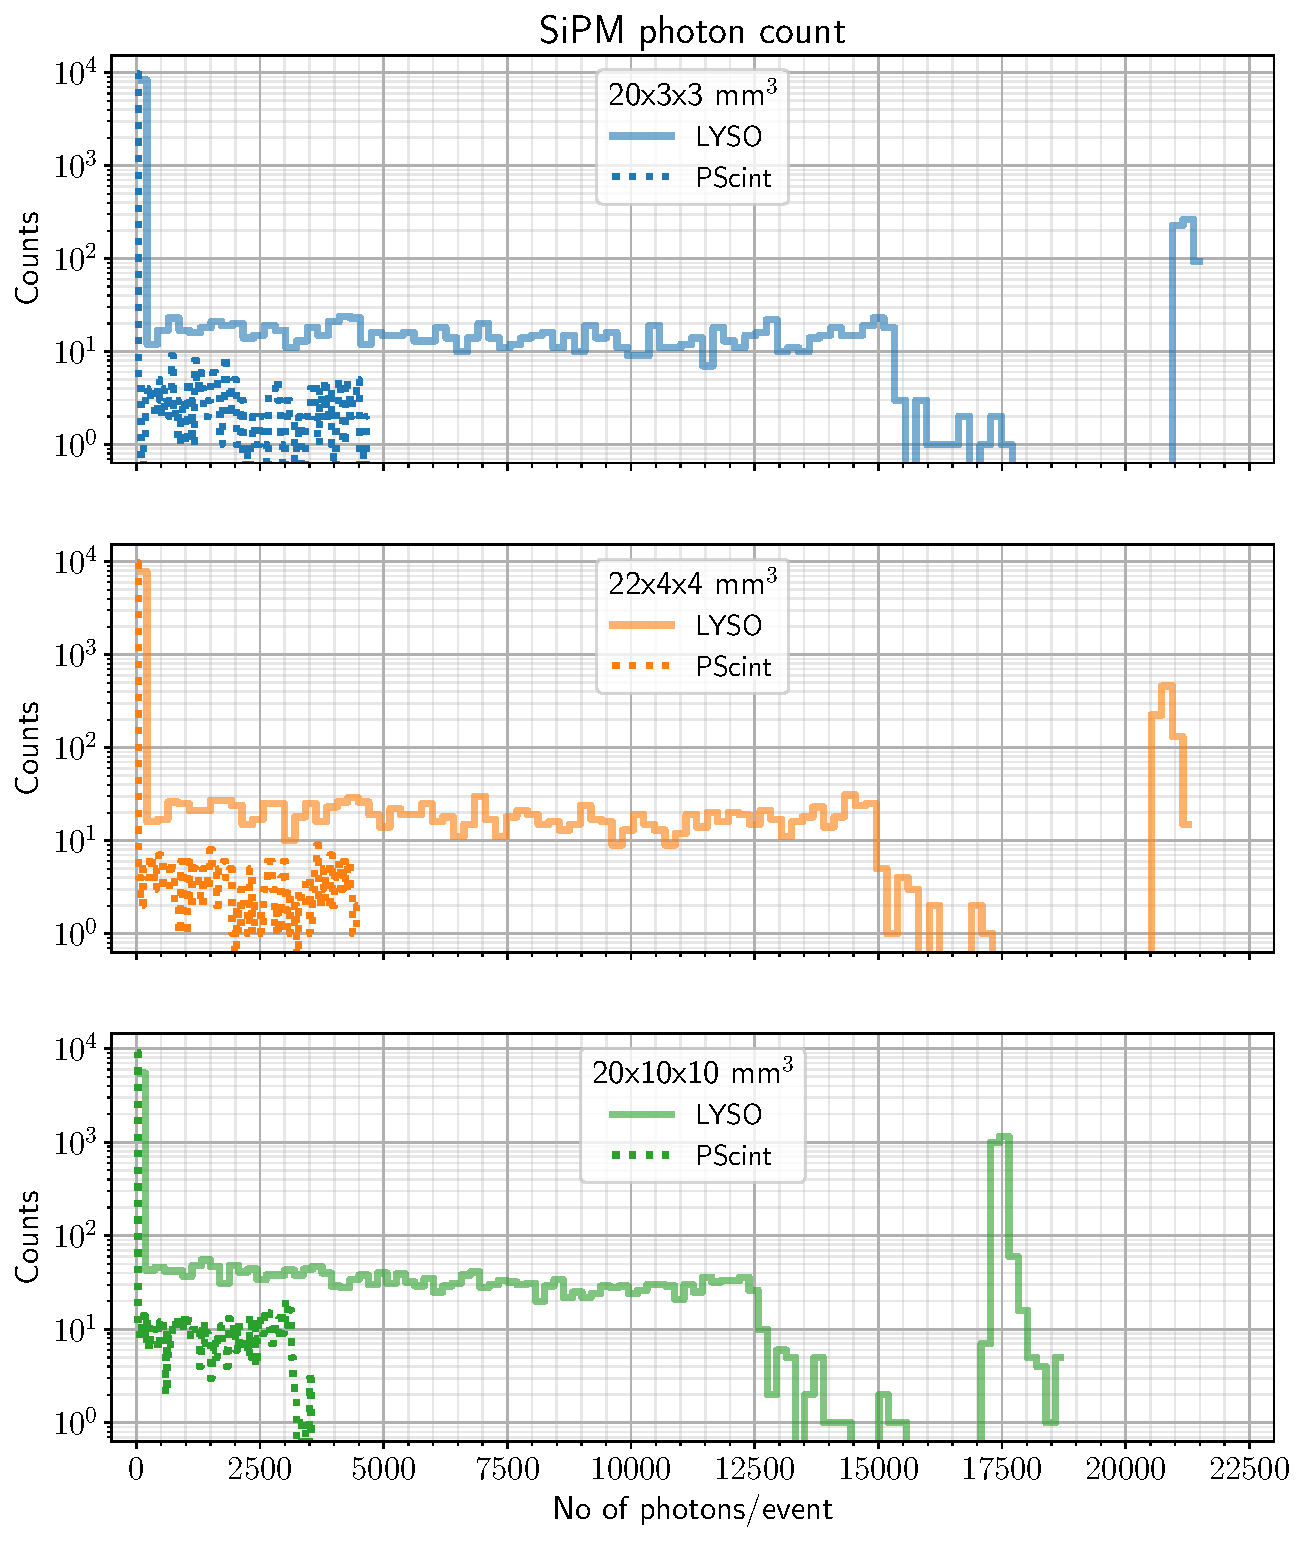
\includegraphics[width=.98\textwidth]{G4_simulations/gammas/run0SiPMphotons.pdf}
  \caption{\label{fig:LYSO_SiPMPhotons}SiPM photon count per event for LYSO and plastic scintillator using three different crystal sizes. In this case the \gps~ shoots 662 \unit{\kilo\eV} gamma-rays.}
\end{figure}


The results shown in Figure \ref{fig:LYSO_SiPMPhotons} are quite important, they clearly show that the photomultiplier collects fewer photons from bigger crystals, which demonstrates that many of them are being attenuated inside the crystal before reaching the SiPM, we know this since no photon can escape the crystal due to the reflective surface used in the simulation. Even more relevant is the steady decrease of photons detected from photoelectric events as the dimensions increase, accompanied by a drop in resolution. In general, it can be seen that plastic scintillator performs poorly compared to LYSO, which is why it is used in this new iteration of CosmicWatches for gamma-ray spectroscopy. Some important results are summarized in tables \ref{tab:sim_results_detection_percentage} and \ref{tab:sim_results_photoelectric_efficiency}.

\begin{table}[H]
  \caption{Simulation results summary for photon detection, measuring the ratio of photons detected vs. produced.}
  \centering
  \begin{tabular}{ c c c }
    \midrule
    \multirow{2}{*}{size [\unit{\mm\cubed}]} & \multicolumn{2}{c}{SiPM counts/Photon production per event [\%]} \\
    & ~~~~~~~~~~~~LYSO & Plastic \\
    \midrule
    $20\times3\times3$ & ~~~~~~~~~~~~97.(6) & 93.9(1) \\
    $22\times4\times4$ & ~~~~~~~~~~~~95.2(7) & 90(2) \\
    $20\times10\times10$ & ~~~~~~~~~~~~80(1) & 65(2) \\
    \bottomrule
  \end{tabular}
  \label{tab:sim_results_detection_percentage}
\end{table}

\begin{table}[H]
  \caption{Simulation results summary for photoelectric detection. This table only shows LYSO results since there were no photoelectric events recorded with plastic scintillators.}
  \centering
  \begin{tabular}{ c c c c}
    \midrule
    LYSO size [\unit{\mm\cubed}] & 662 \unit{\kilo\eV} events & Photon production/event & SiPM counts/event \\
    \midrule
    $20\times3\times3$ & 583 & $21864\pm 7$ & $21226\pm 118$ \\
    $22\times4\times4$ & 831 & $21863\pm 7$ & $20821\pm 124$ \\
    $20\times10\times10$ & 2253 & $21861\pm 7$ & $17474\pm 116$ \\
    \bottomrule
  \end{tabular}
  \label{tab:sim_results_photoelectric_efficiency}
\end{table}